\documentclass[11pt]{article}
\usepackage{graphicx}
\usepackage{hyperref}
\usepackage{caption}
\usepackage{amsmath}
\usepackage{mathtools}
\usepackage{physics}
\newcommand{\numpy}{{\tt numpy}}    % tt font for numpy

\topmargin -.5in
\textheight 9in
\oddsidemargin -.25in
\evensidemargin -.25in
\textwidth 7in

\begin{document}

% ========== Edit your name here
\author{Hongqing Liu, hl85}
\title{CS 498: Assignment 3: Iterative Closest Point and Odometry}
\date{March 20, 2023}
\maketitle

\medskip


\section*{Submission}
In this assignment, you will code your own point cloud alignment and depth odometry algorithm to estimate camera poses and build 3D maps of the environment through raw depth observation. The starter code consists of 2 python files you will modify along with a folder of some images and metadata. Please put together a single PDF with your answers and figures for each problem, and submit it to Gradescope (Course Code: BBX6NE). If your code produces figures they should go in this pdf, along with a description of what you did to solve the problem. We recommend you to use the latex template files we provided. For code submission, make sure you upload the provided ``.py" files with your modifications. The graders will check both your PDF submission and your code submission if needed. 

\section*{Iterative Closest Point} 

In this part, your task is to align two point clouds. The algorithm we will leverage is called iterative closest point (ICP). There are several components. 

\paragraph{Question 1 (Unprojection)[1 pts]:} Here, you will be modifying the function ``rgbd2pts" in ``icp.py". Given the input RGB-D image and the intrinsic matrix, your task is to unproject the RGB-depth image observations back to 3D in the form of a colored point cloud. We provide an open3d visualization for the point cloud and you should report the resulting figure in the document. Please avoid solutions using for-loop or directly calling an off-the-shelf unprojection function.

\textbf{Answer: } The unprojection result is shown as follows:
\begin{center}
    \small
    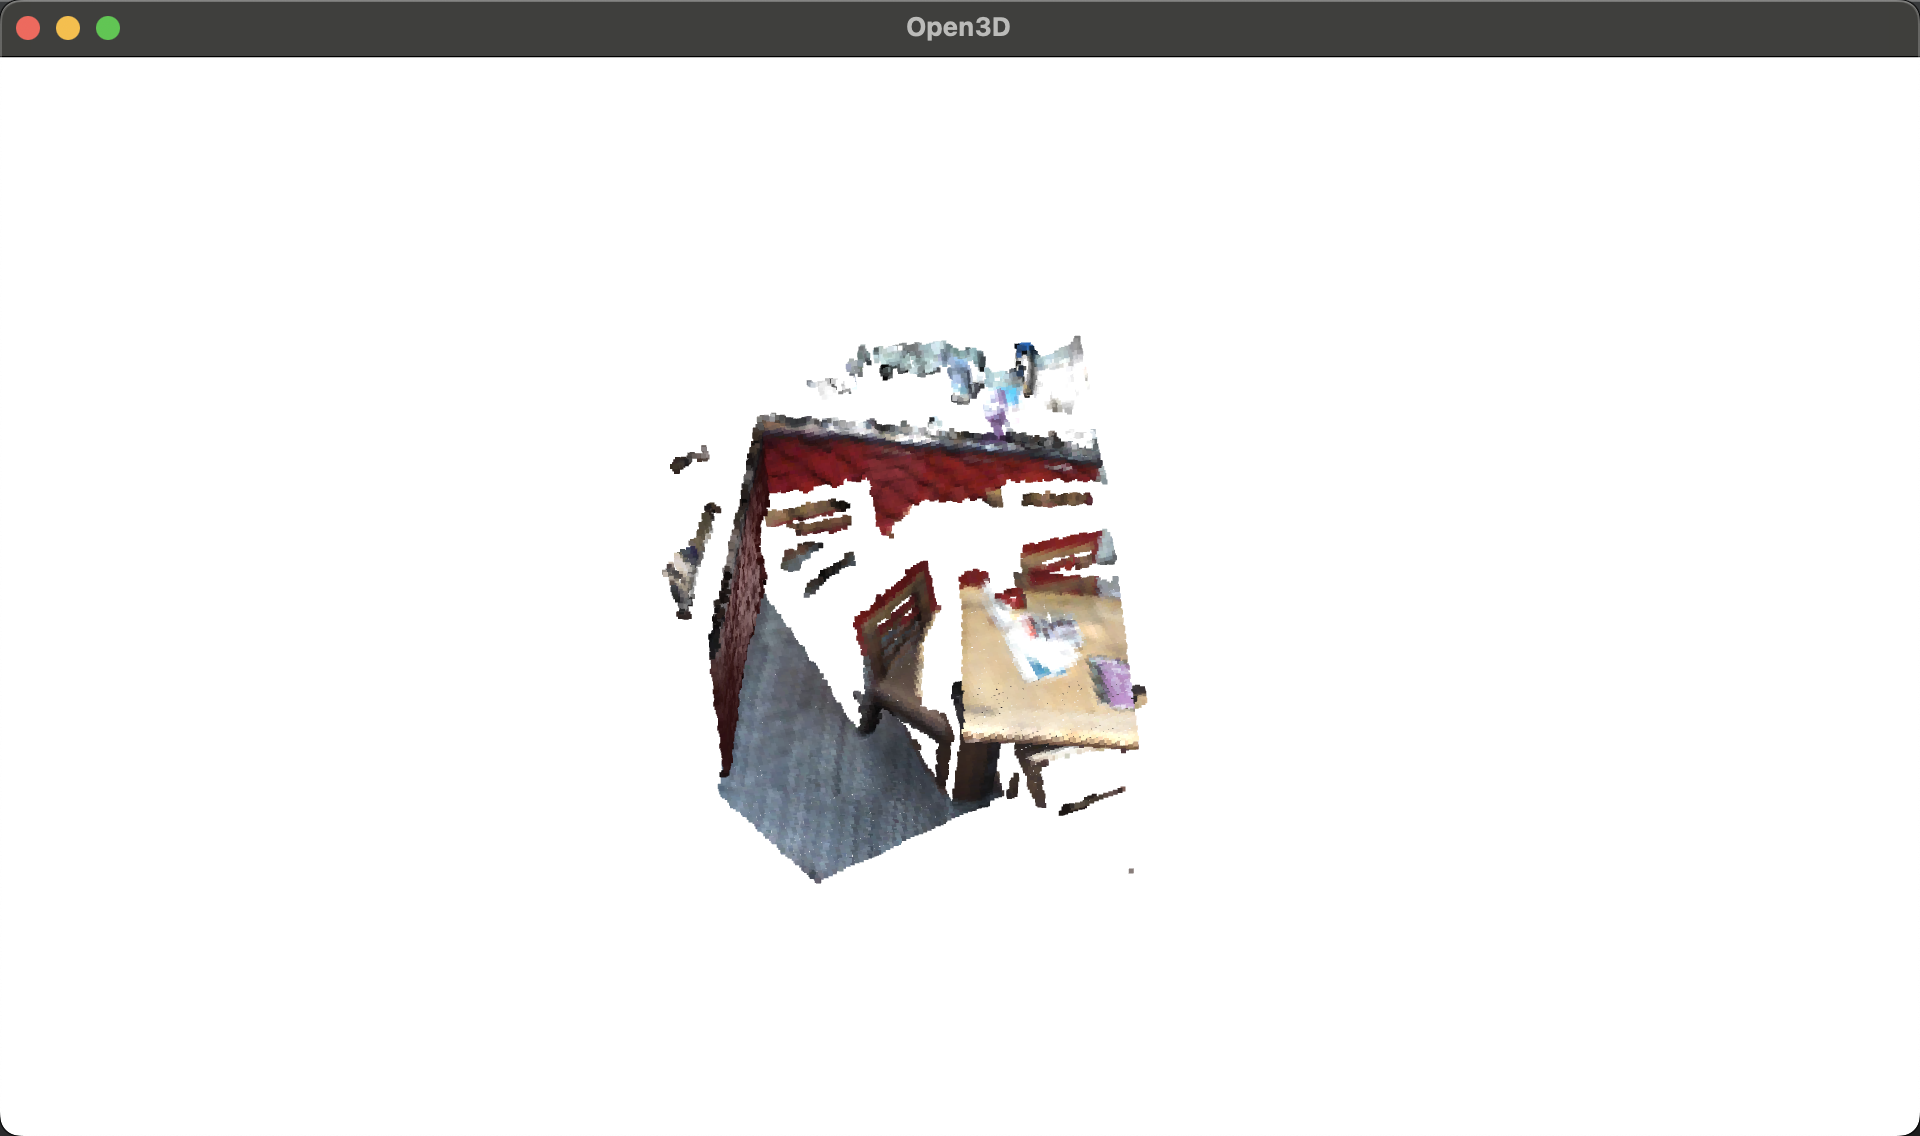
\includegraphics[width=0.3\linewidth]{fig/Q1output1.png}
    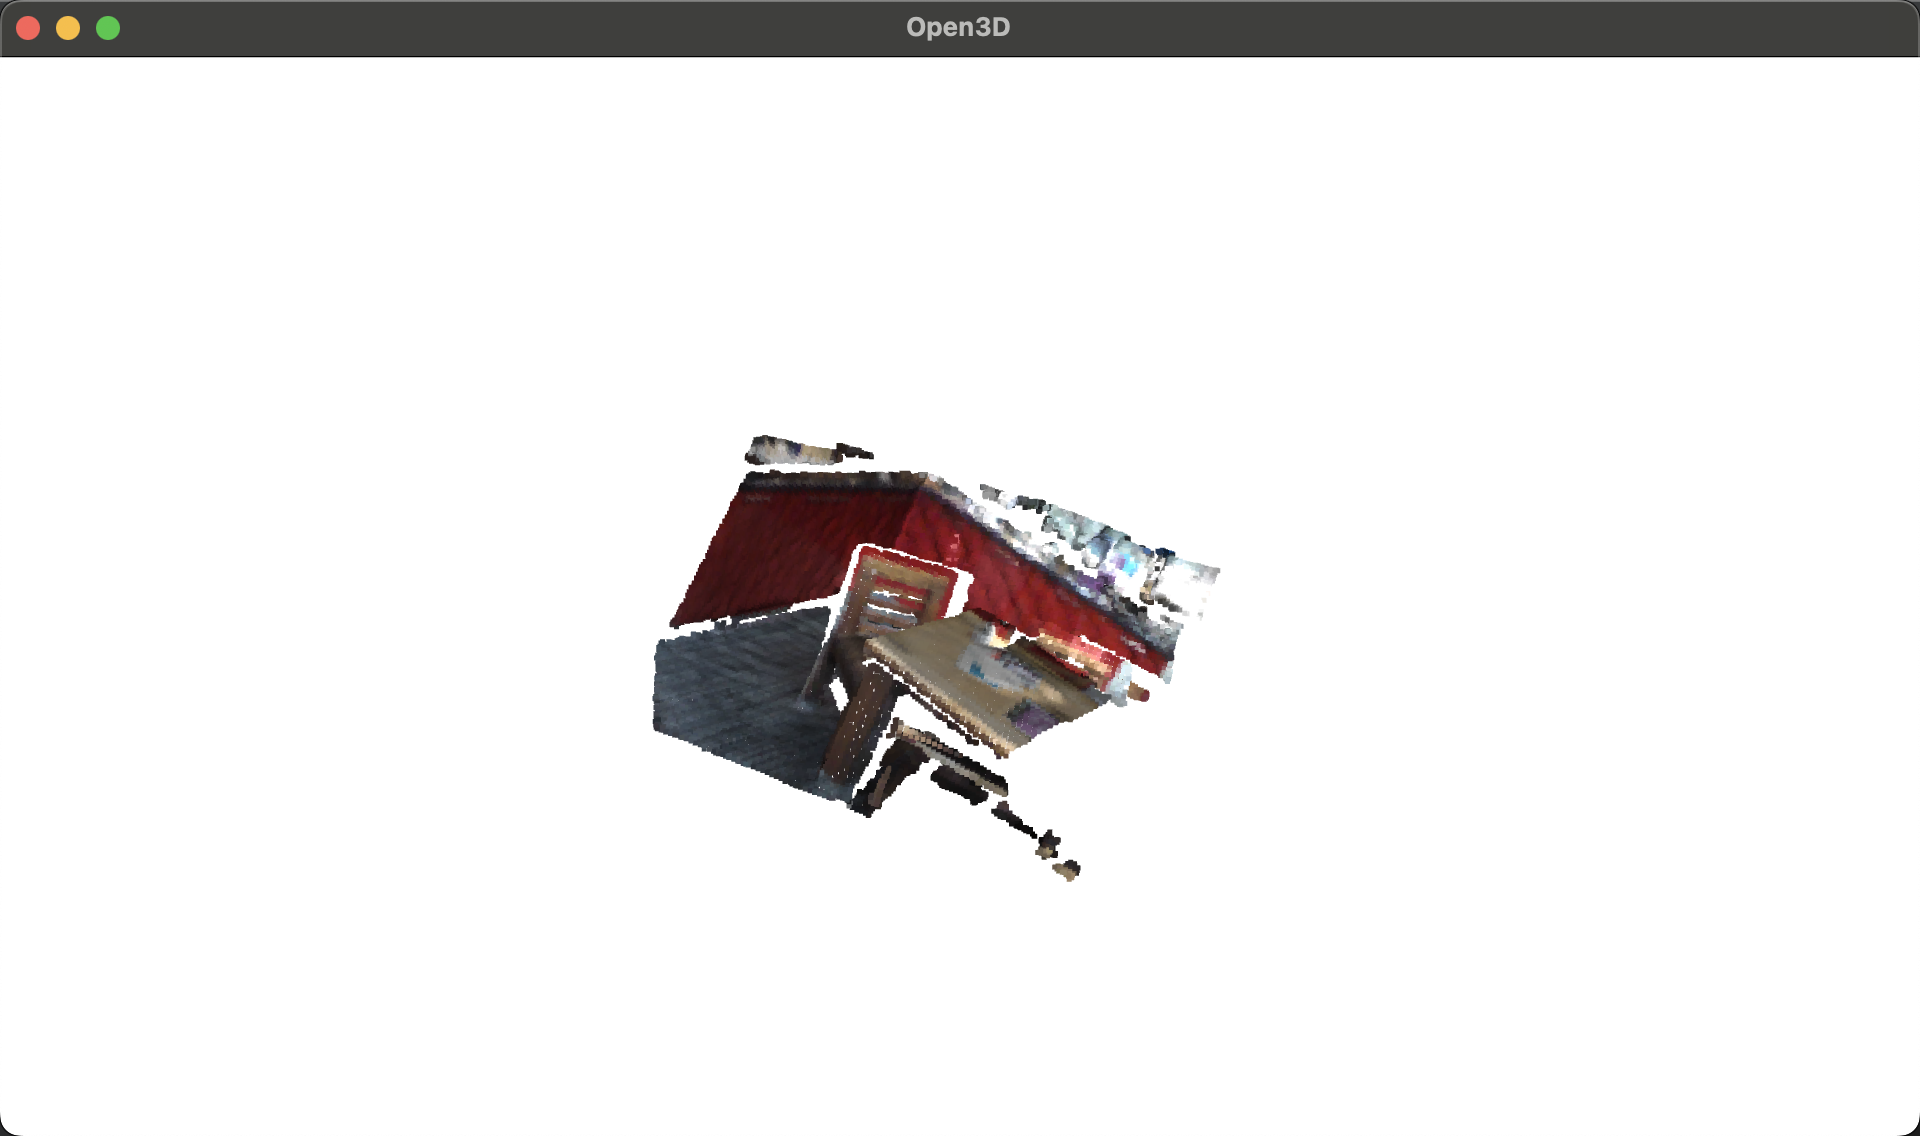
\includegraphics[width=0.3\linewidth]{fig/Q1output3.png}
    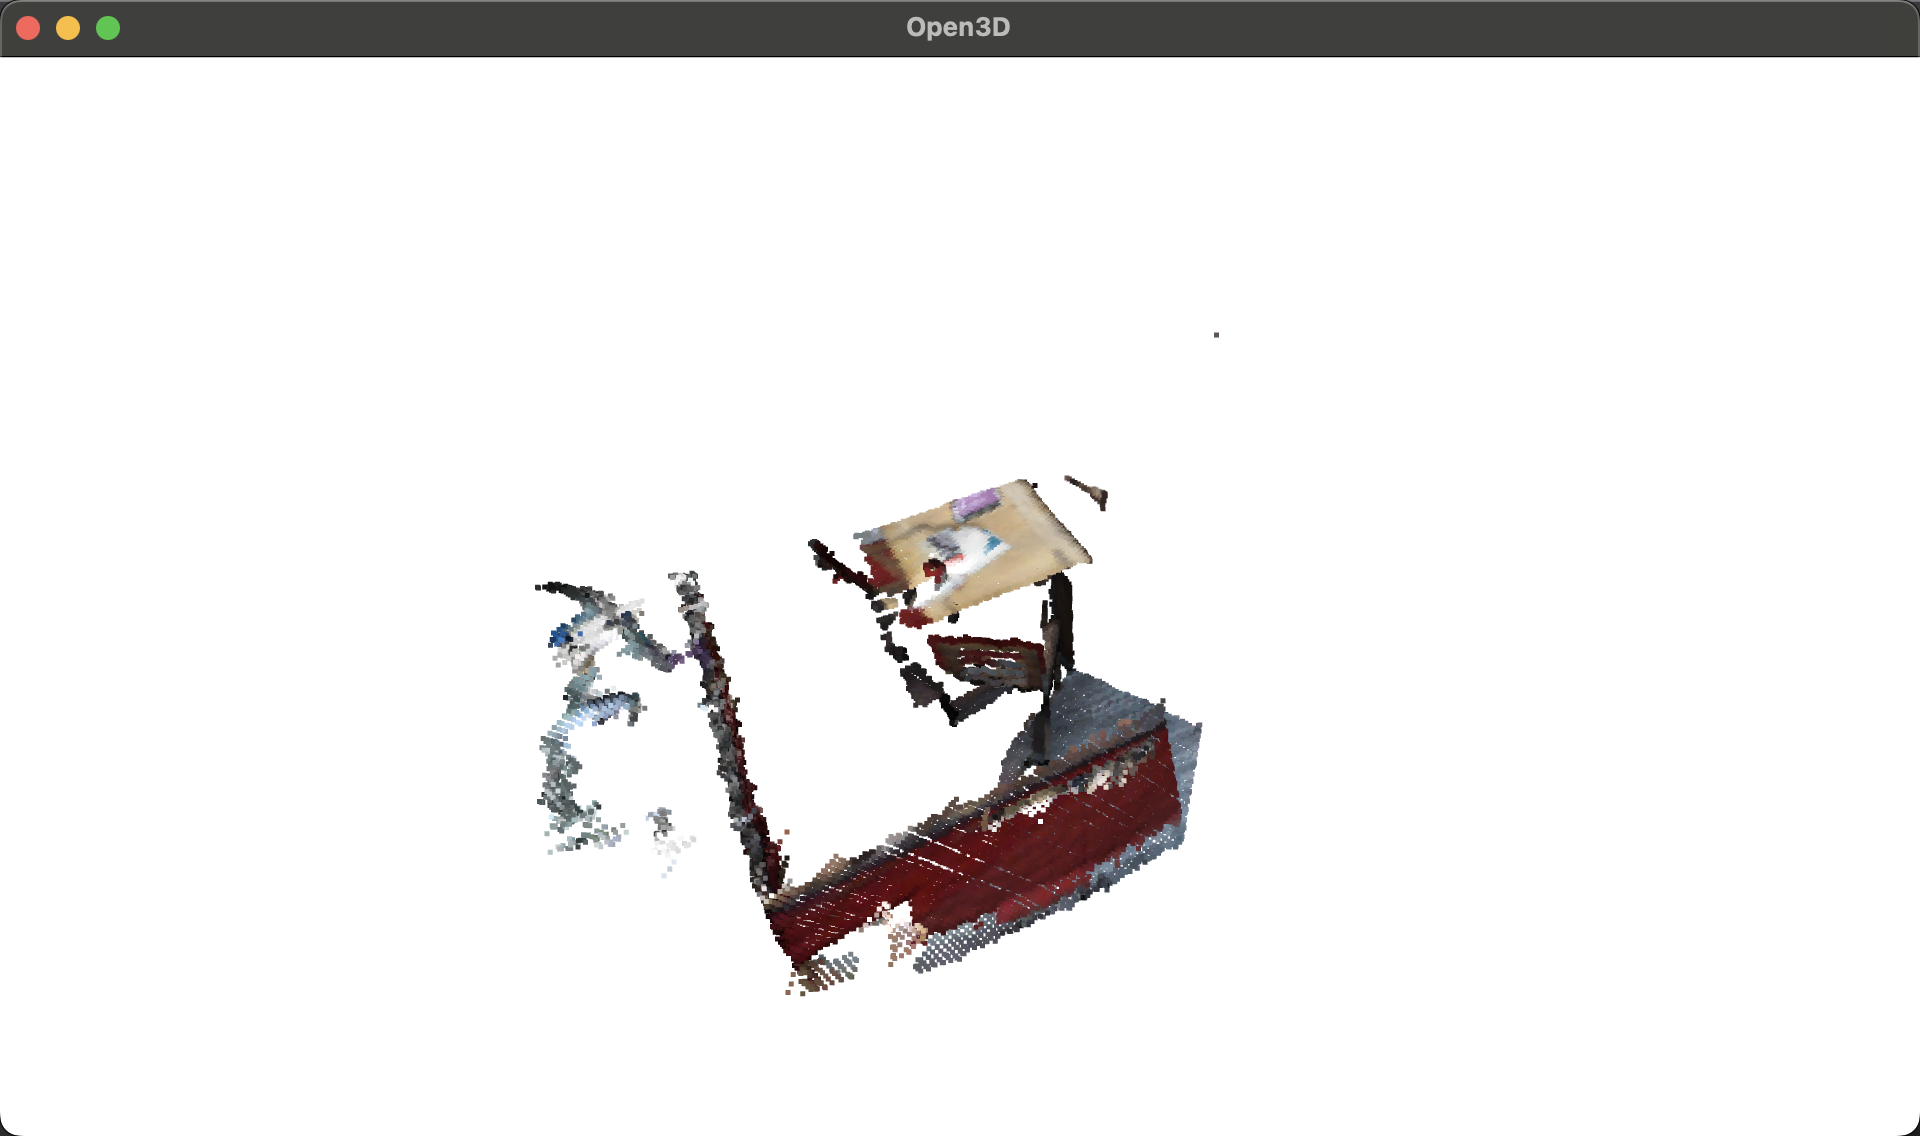
\includegraphics[width=0.3\linewidth]{fig/Q1output2.png}
\end{center}
\paragraph{Question 2 (Rigid Transform Fitting) [3 pts]:} Here, you will be modifying the function ``fit\_rigid" in ``icp.py". For this question, your task is to implement the rigid transformation fitting algorithm, assuming you are given N pairs of corresponding 3d points. You should refer to our lecture slide on depth sensing, and additional references could be found here: \href{https://www.ltu.se/cms_fs/1.51590!/svd-fitting.pdf}{link1}, \href{https://igl.ethz.ch/projects/ARAP/svd_rot.pdf}{link2}, \href{https://en.wikipedia.org/wiki/Orthogonal_Procrustes_problem}{link3}. You will use the point-to-point distance in this part. 
In addition, please provide an answer and necessary mathematical justification on what will happen if the input corresponding point pair contains errors and whether you could identify such a situation. 

\textbf{Answer: } When we want to find the rigid transform that minimize the average distance between two set of point cloud using point-to-point distance, we firstly calculation translation matrix by align the center of two cloud points, then we need to find optimal rotation matrix between two certer-normalized point cloud.

The code of point-to-point rigid transform is shown as follows:
\begin{center}
    \small
    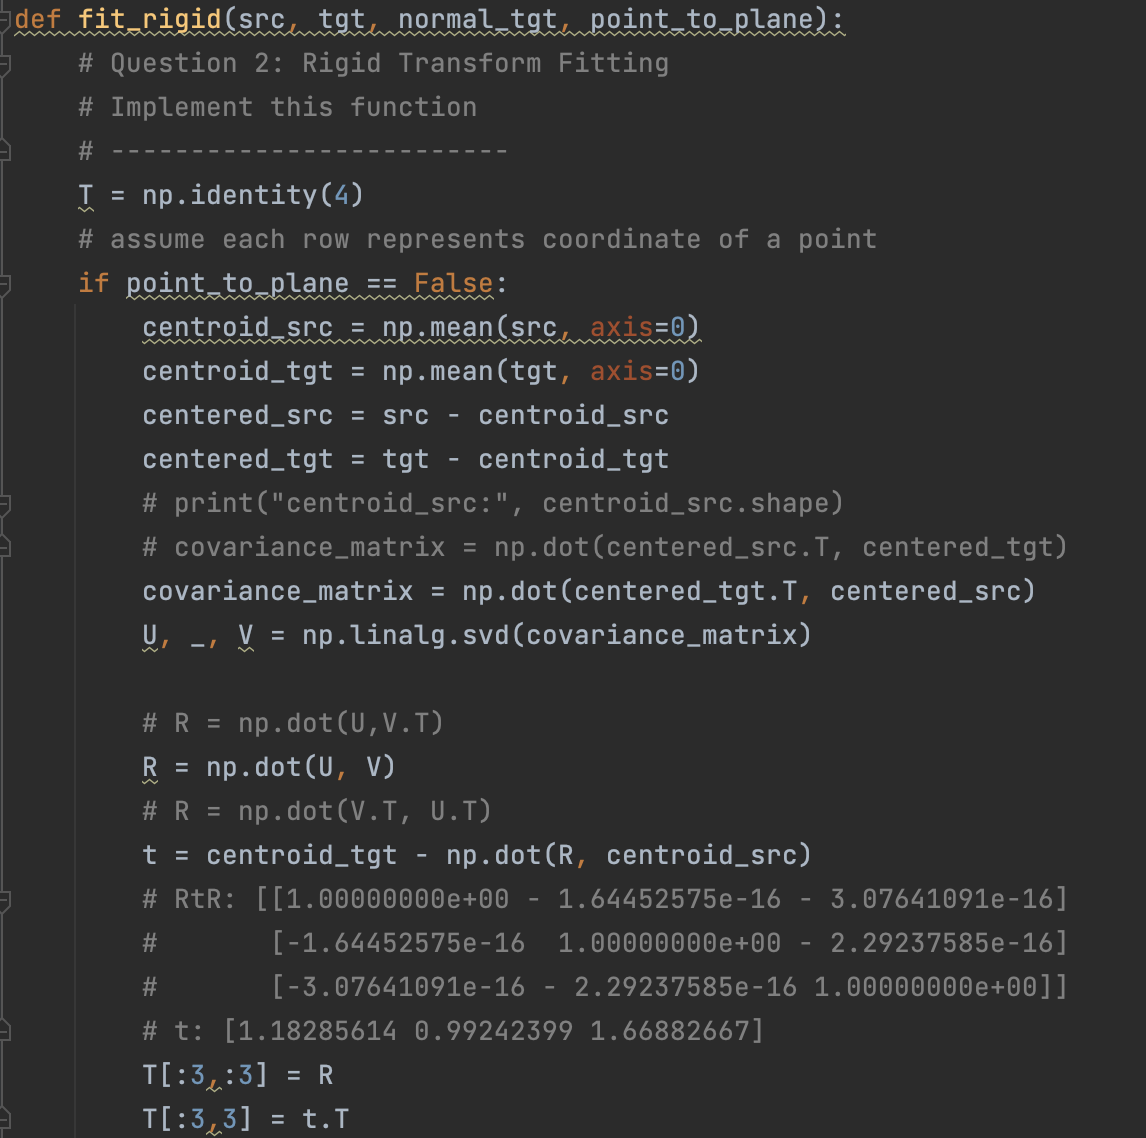
\includegraphics[width=0.5\linewidth]{fig/Q2code.png}
\end{center}
Here you can find that if the input corresponding point pair contains errors, the resulting rigid transformation will not accurately align the two point sets.

There are two kinds of error in this situation. One common type of error is an outlier, which is a point that does not belong to the corresponding pair. Outliers can significantly affect the computation of the rigid transformation, as they can introduce large errors in the covariance matrix. The outlier will significantly effect the rotation matrix as the rotation matrix is calculated based on the SVD of covariance matrix, it will also effect the translation matrix since the outlier can effect the center of the cloud points.

The other kind of error is caused by mismatches. Mismatches can also affect the computation of the rigid transformation, as they can lead to a rotation matrix that does not accurately align the two point sets. Mismatches always occurs when two point cloud are far away or need huge rotation. However, in this case, we are align different cloud points between each frame, they are very close to each other.

To identify those errors, we can compute residual error after rigid transformation. If it's large, it shows we have corresponding error. However, since those problems are not significant in this situation, I do not add this ``error identification'' part in the code.

\paragraph{Question 3 (Point-to-Point ICP Loop) [3 pts]:} Here you will be modifying the function ``icp" in ``icp.py". Your task is to complete the full ICP algorithm. You are provided a starter code with hints in the comments. Please complete it and try to align the provided two point clouds. We provide a visualization for the aligned results which includes your estimated camera poses compared to the GT camera poses. Please provide an image of the final visualization in this pdf along with a description of the algorithm.

\textbf{Answer: } Here is a brief description of ICP.
In each iteration, we basically have two steps. In the first step, I find the corresponding points between two point cloud based on K-d tree and assign each source point to the corresponding target point. Then I use rigid transform function to align two point clouds.

The code of ICP and image of final visualization are shown as follows:
\begin{center}
    \small
    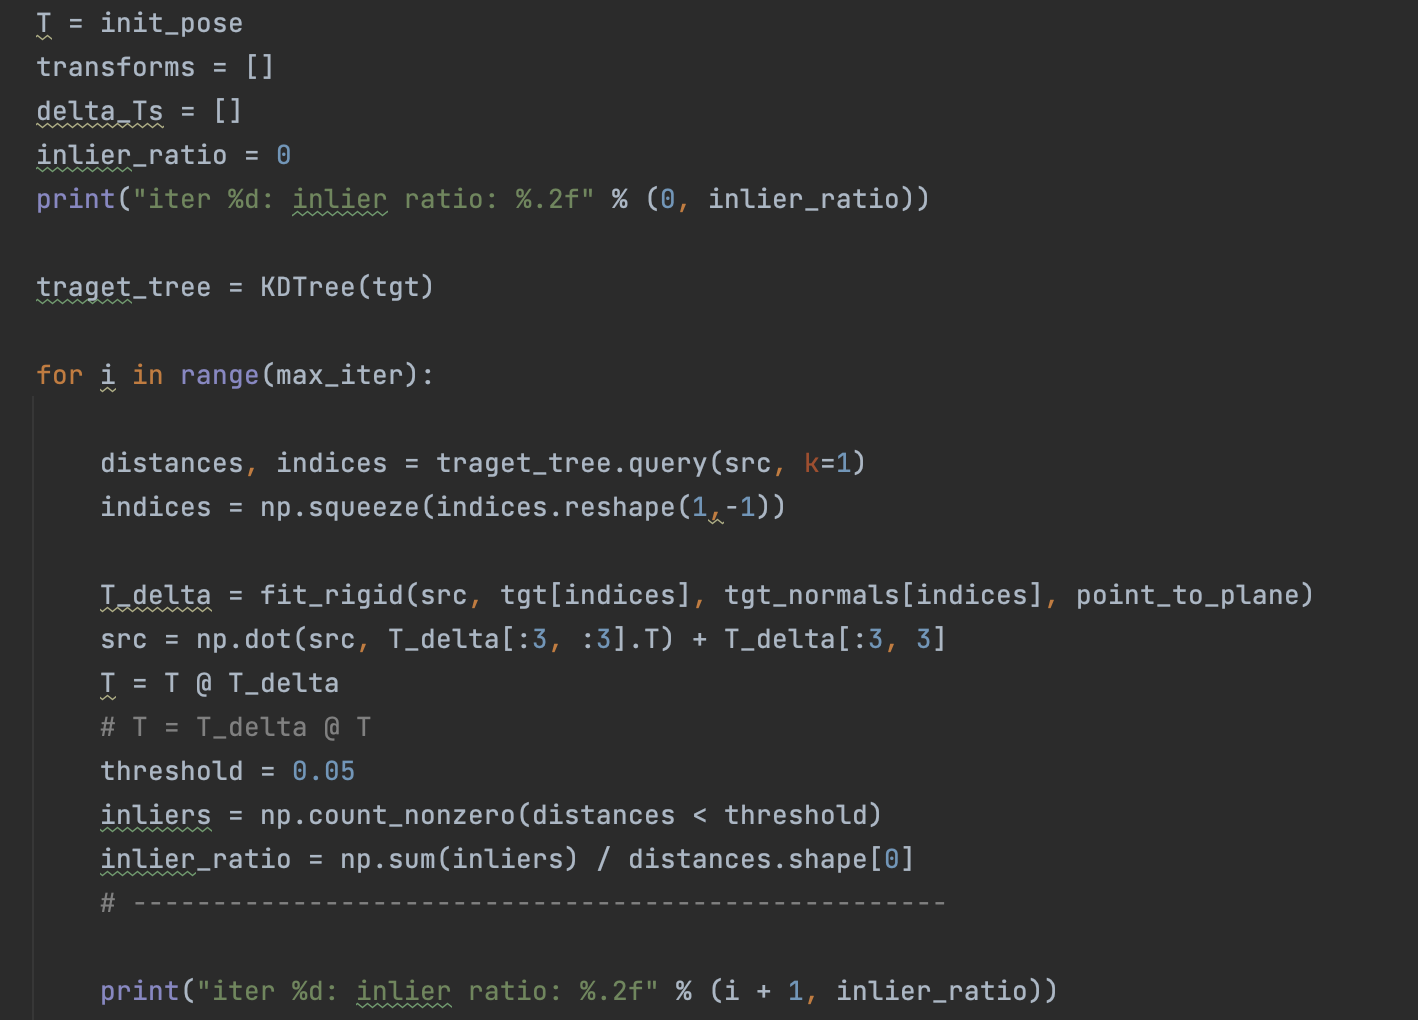
\includegraphics[width=0.3\linewidth]{fig/Q3code.png}
\end{center}
\begin{center}
    \small
    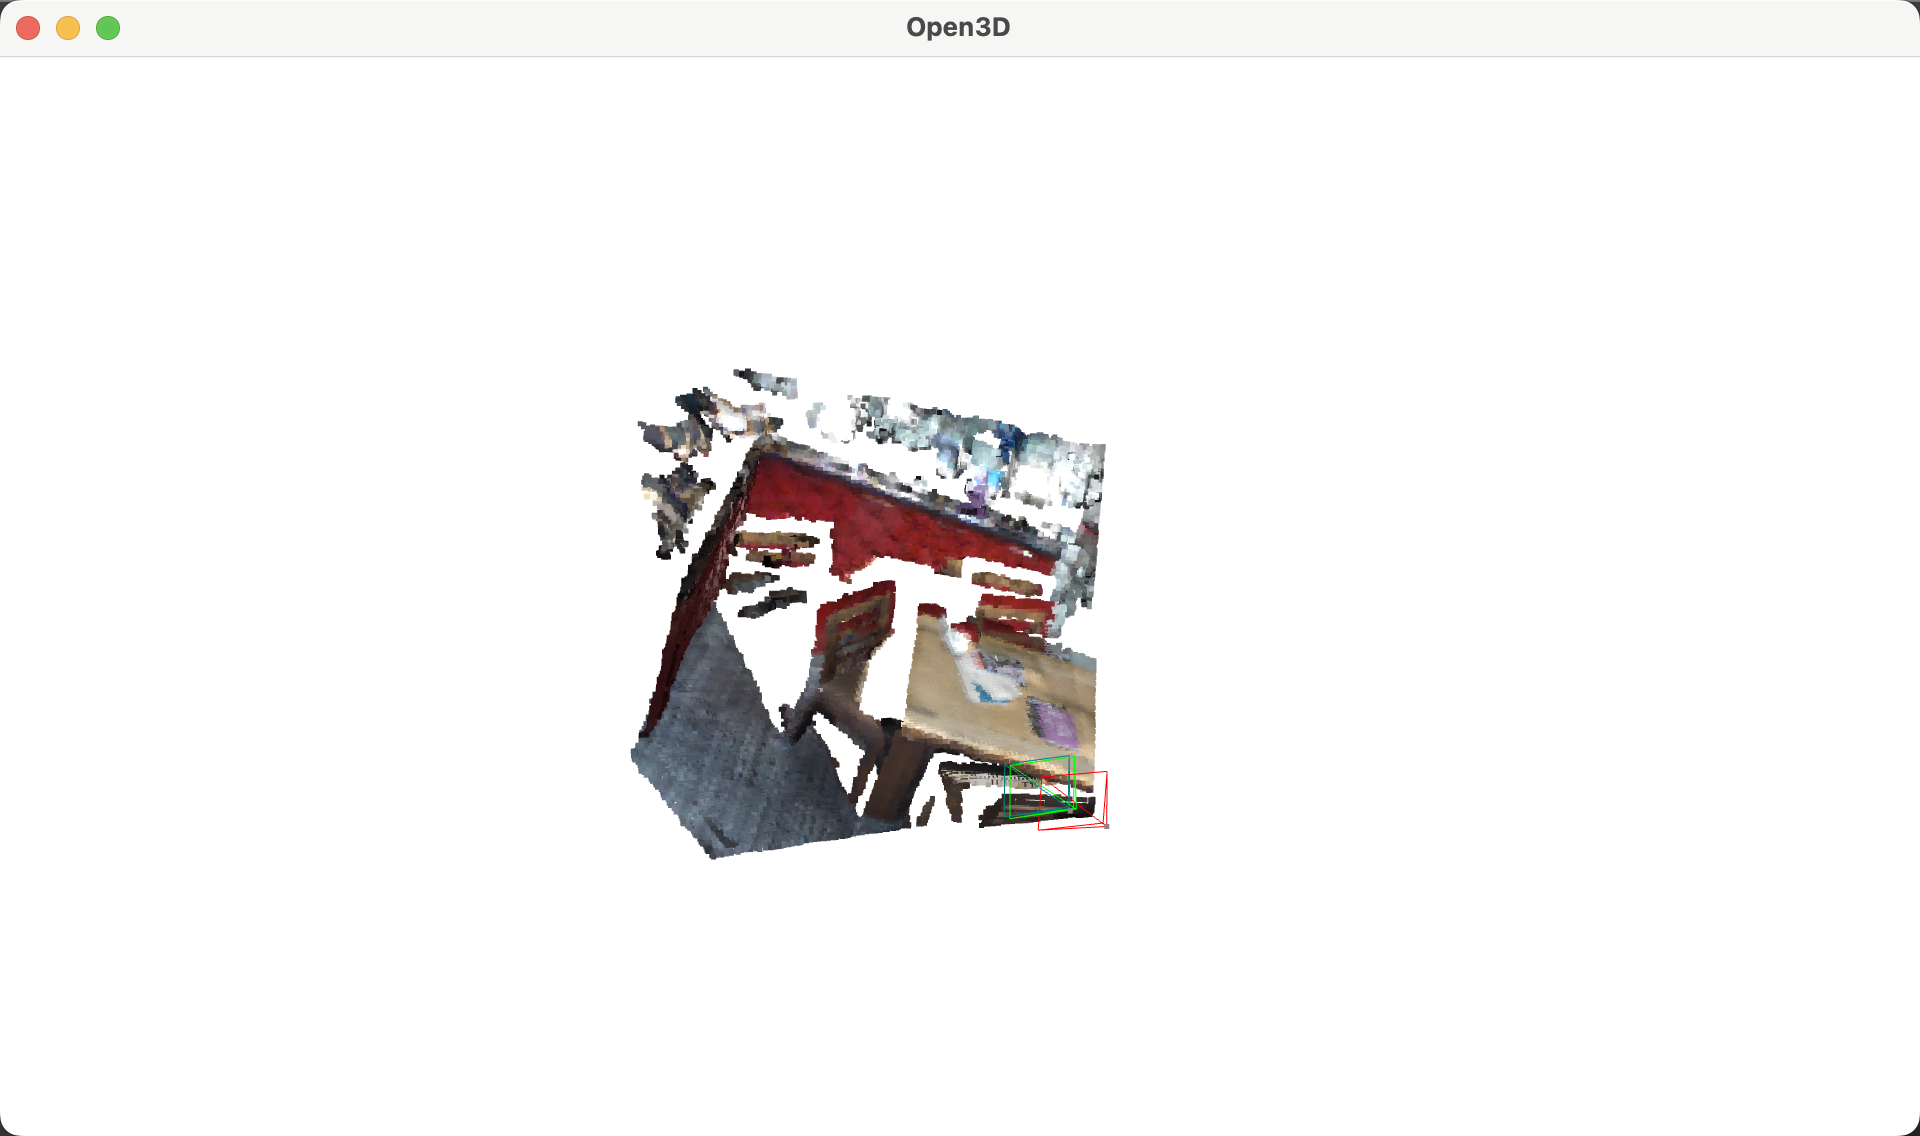
\includegraphics[width=0.3\linewidth]{fig/Q3output1.png}
    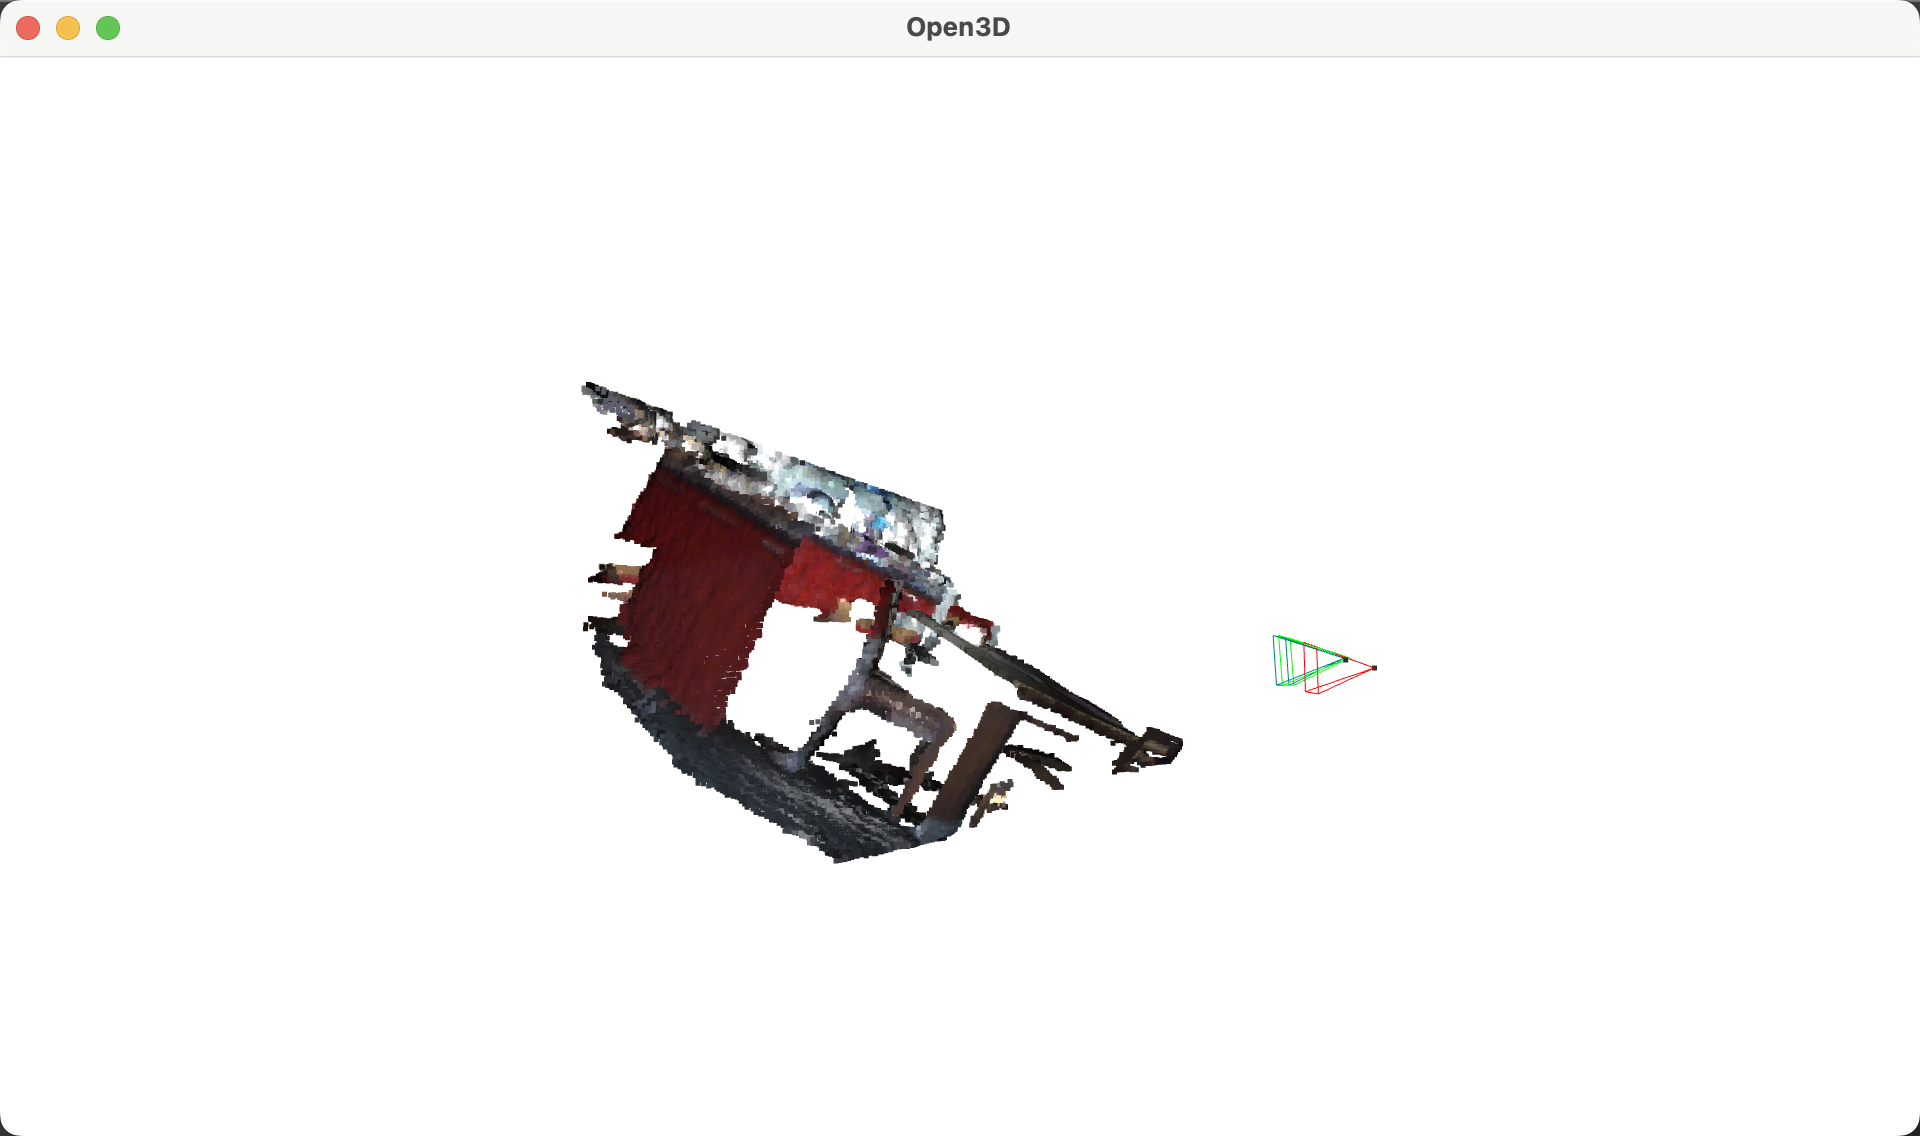
\includegraphics[width=0.3\linewidth]{fig/Q3output2.png}
    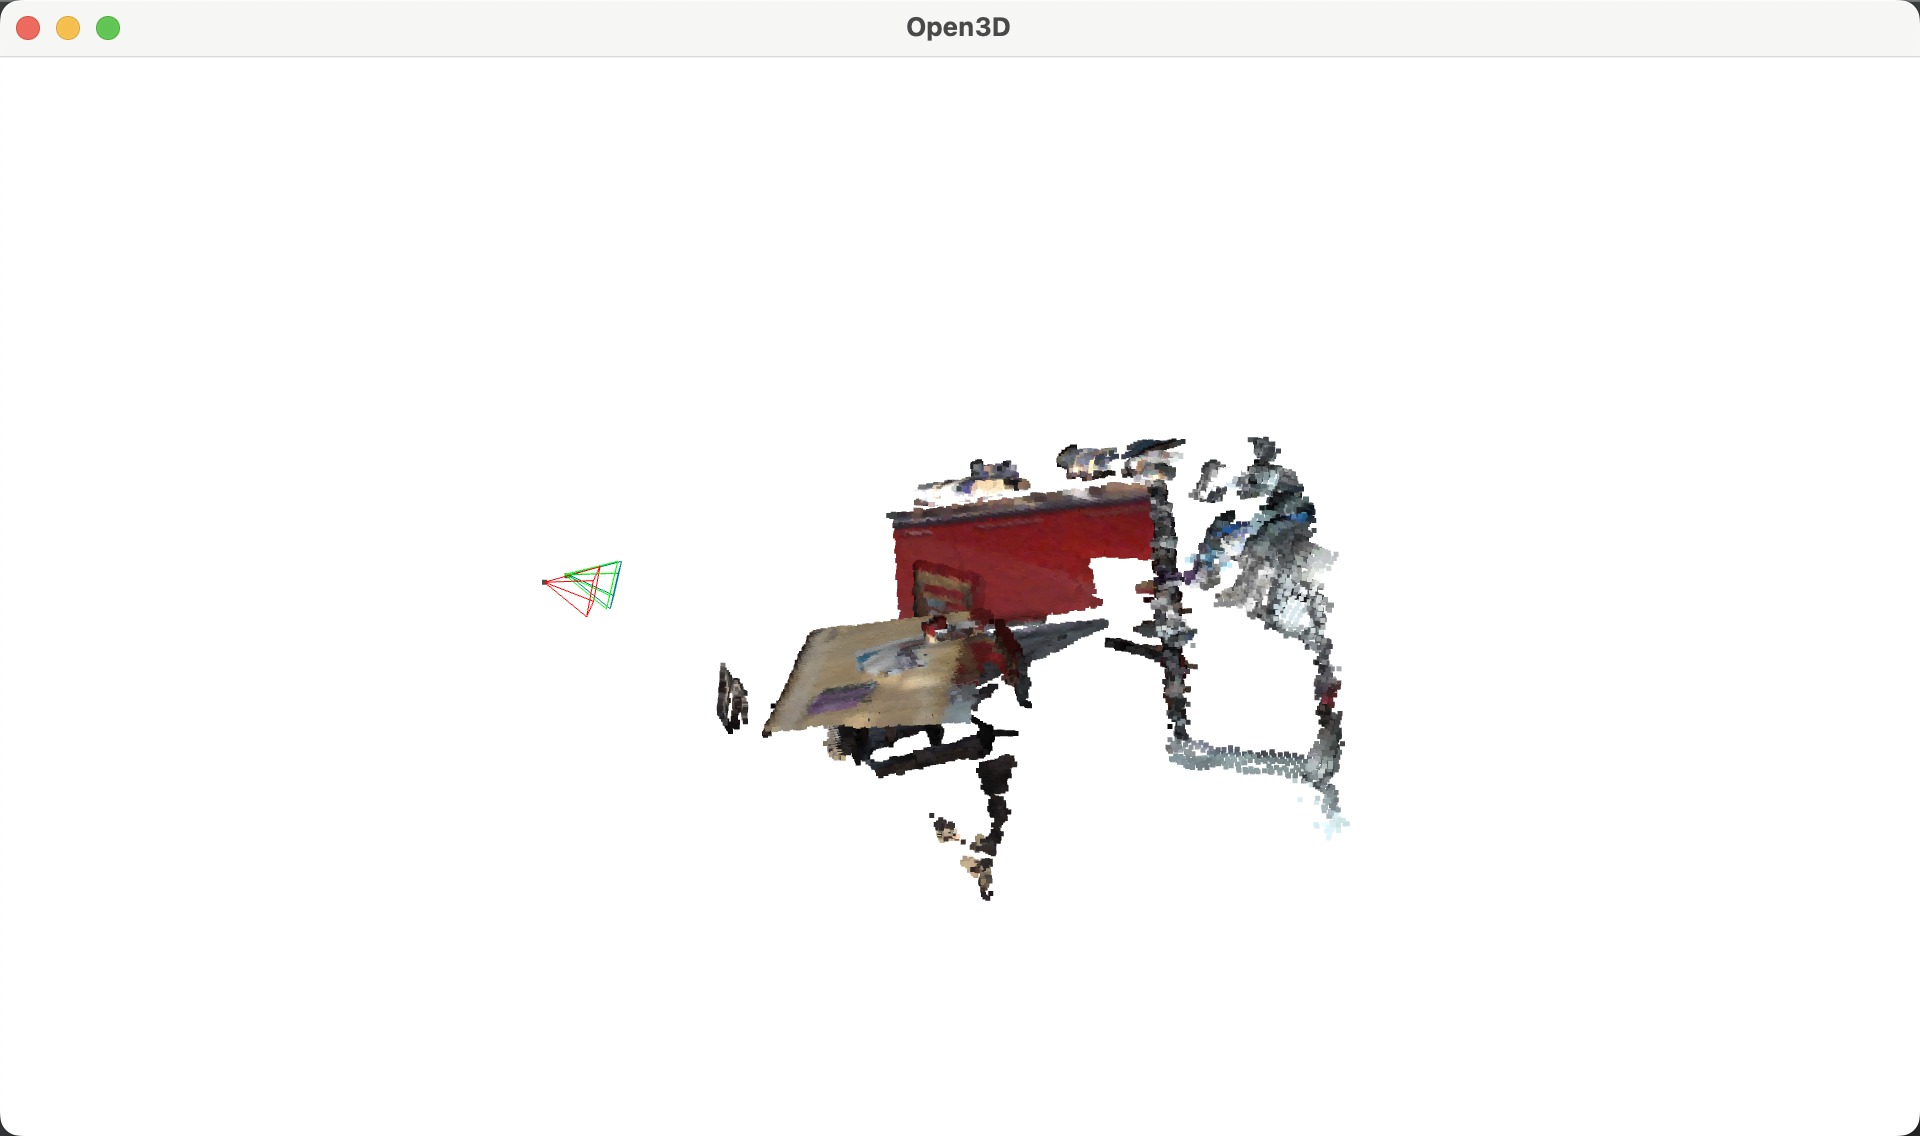
\includegraphics[width=0.3\linewidth]{fig/Q3output3.png}
\end{center}
\paragraph{Question 4 (Point-to-Plane ICP) [2 pt]:} Here you will be modifying ``icp.py". Please extend your point-to-point ICP to allow it to take point-to-plane distance. Please run the alignment on your testing cases again and visualize the alignment results. Please justify when point-to-plane might be preferred over point-to-point distances (provide mathematical justification if necessary). 

\textbf{Answer: }The Point-to-Plane ICP algorithm iteratively minimizes the sum of squared distances between the source points and their corresponding planes in the target point set. The code of point-to-plane rigid transform is shown as follows:
\begin{center}
    \small
    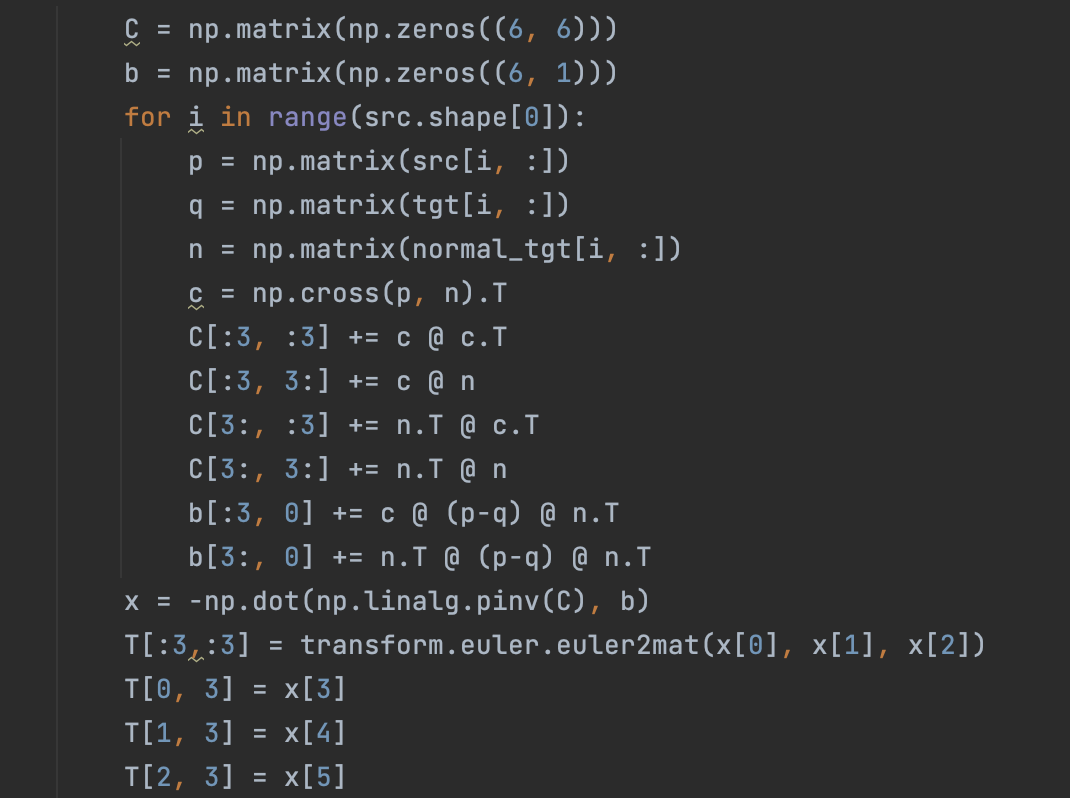
\includegraphics[width=0.3\linewidth]{fig/Q4code.png}
\end{center}
It takes source points, target points, and target normals as input and ouput the transform matrix.

The alignment results are shown as follows:
\begin{center}
    \small
    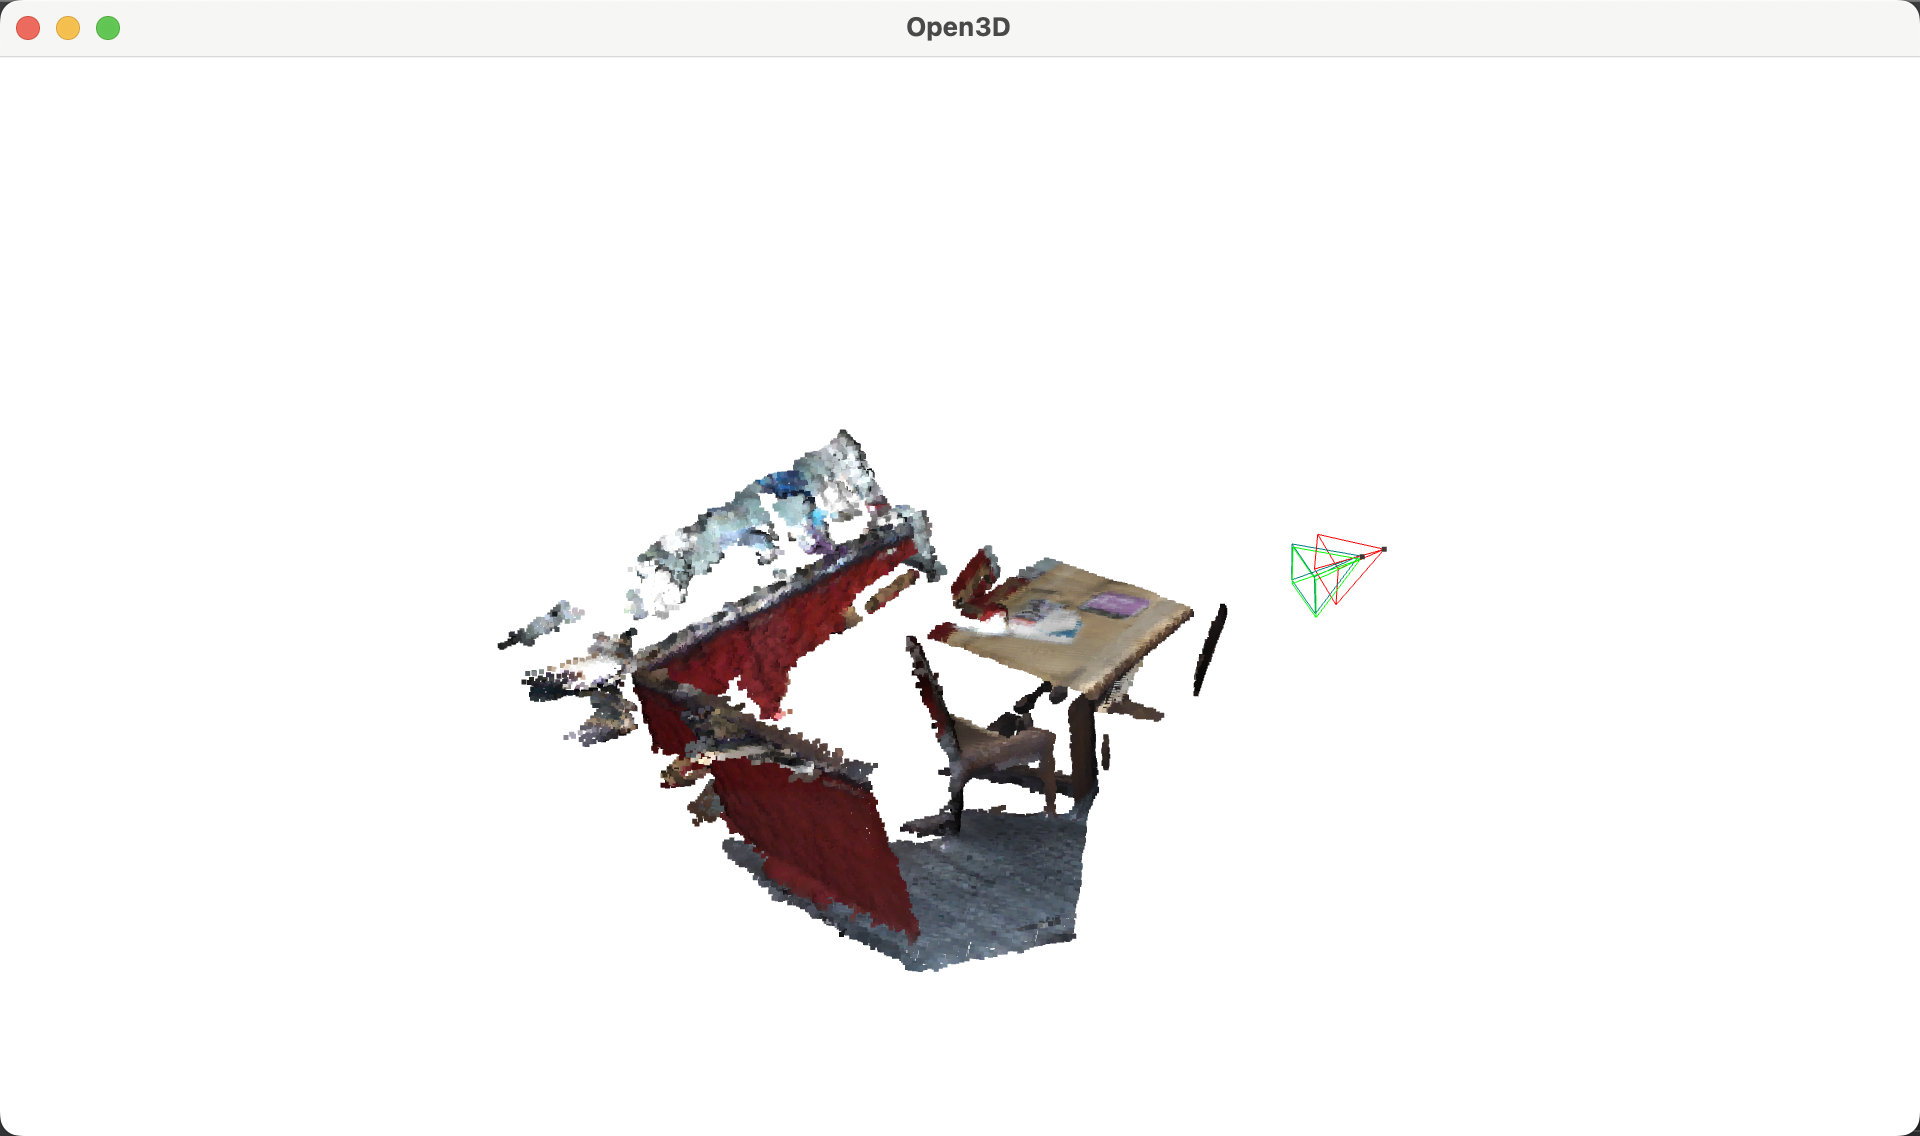
\includegraphics[width=0.3\linewidth]{fig/Q4output1.png}
    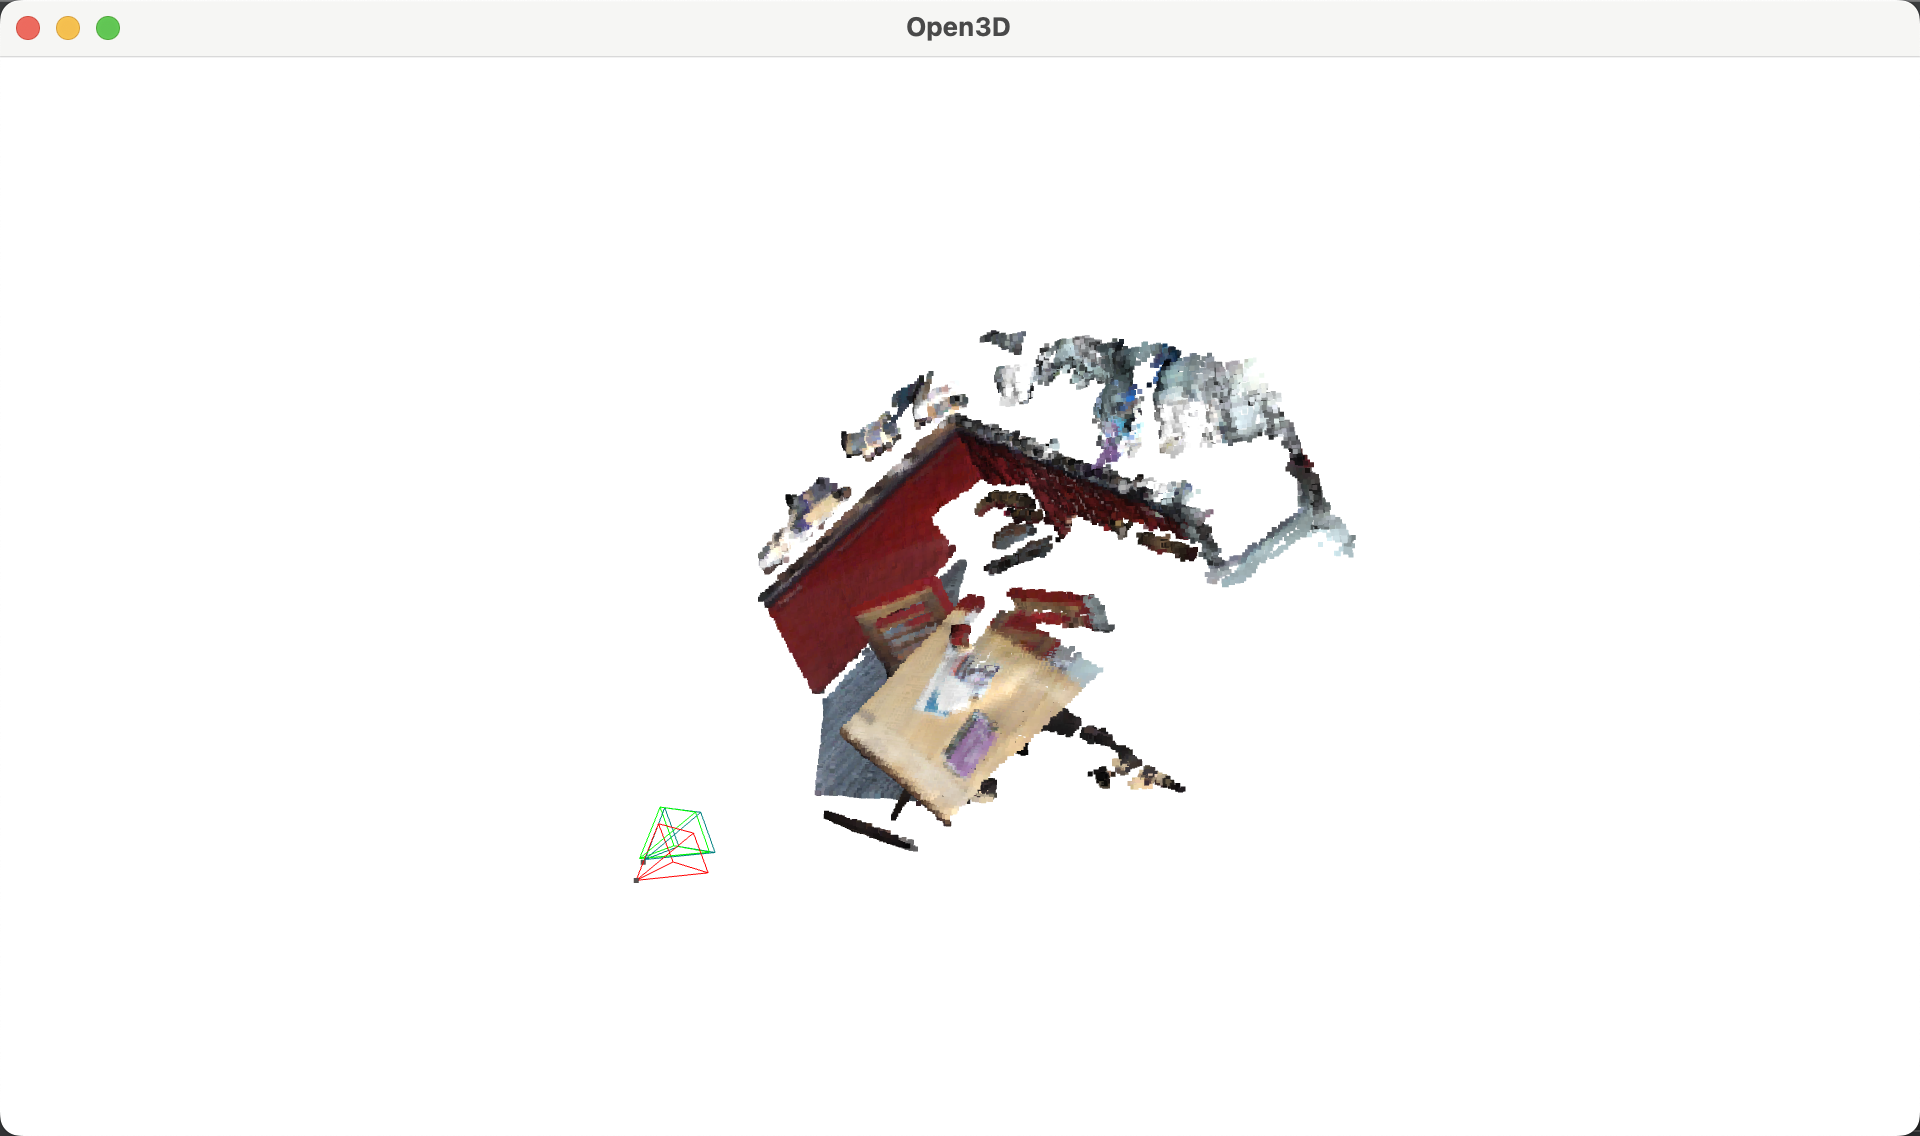
\includegraphics[width=0.3\linewidth]{fig/Q4output2.png}
    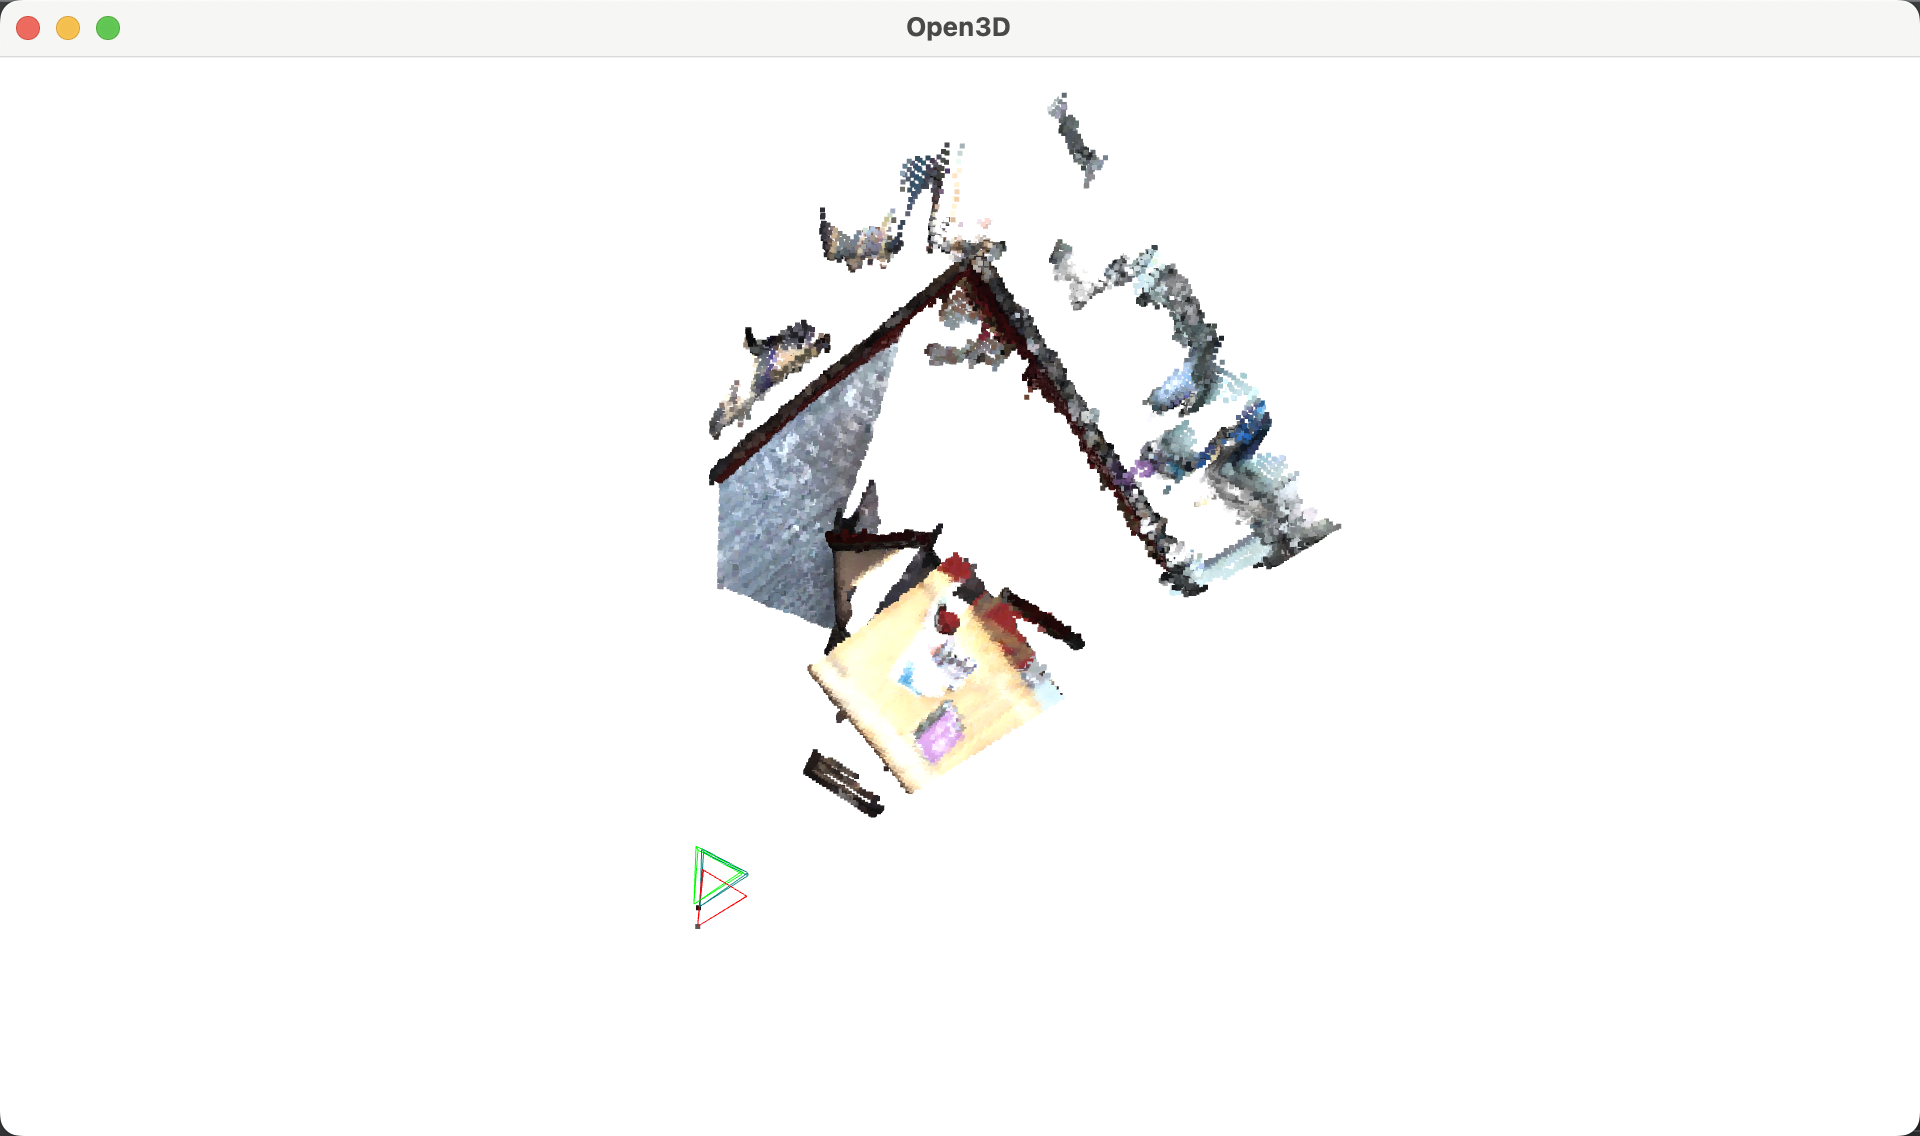
\includegraphics[width=0.3\linewidth]{fig/Q4output3.png}
\end{center}
When the surface of the target object is smooth, point to plane ICP has better performance. To be specific, it takes the orientation of the surface at each point into accout so that it has less chance to be influence by the outliers and converge to local minimum. On the other hand, if the surface of target is rough and has sharp features, point-to-point ICP may have better performance. 

\paragraph{Question 5 (Translation and Rotation Error) [1 pt]:} Now, we would like to evaluate how good our estimated poses are. Unlike other prediction tasks where the output is categorical data or euclidean vectors, pose estimation lies in SE(3) space. And we might want to evaluate rotation and translation components separately. Please check this reference and implement the translation and rotation error defined in Eq. 5-6. (\href{https://cmp.felk.cvut.cz/~hodanto2/data/hodan2016evaluation.pdf}{link}). Please report your translation and rotation errors for the two ICP algorithms, along with the estimated and gt pose.  

Here is the groud truth pose, estimated pose and rotation/translation error of point-to-plane ICP:

gt pose:
$$\begin{bmatrix}
    0.99833244 & -0.03859617 & 0.04303848 & 0.05789683\\
    0.0402418 & 0.99846981 & -0.03803178 & 0.0360833\\
    -0.04150506 & 0.03970066 & 0.9983549 & -0.06788991\\
    0 & 0 & 0 & 1    
\end{bmatrix}$$

estimated pose:
$$\begin{bmatrix}
    0.9977769 & -0.04188976 & 0.05183158 & 0.03027317\\
    0.04365268 & 0.9984896 & -0.03336095 & 0.03344404\\
    -0.05035581 & 0.03554937 & 0.99809846 & -0.0723181\\
    0 & 0 & 0 & 1
\end{bmatrix}$$

rotation/translation error:
$$\begin{bmatrix} 0.00971669 & 0.02810056 \end{bmatrix}$$

Here is the groud truth pose, estimated pose and rotation/translation error of point-to-point ICP:

gt pose:  
$$\begin{bmatrix} 
    0.99833244 & -0.03859617 & 0.04303848 & 0.05789683 \\
    0.0402418 & 0.99846981 & -0.03803178 & 0.0360833 \\
    -0.04150506 & 0.03970066 & 0.9983549 & -0.06788991 \\
     0 & 0 & 0 & 1 \\
\end{bmatrix}$$

estimated pose:  
$$\begin{bmatrix} 
    0.99872813 & -0.03824255 & 0.03285785 & 0.07139511 \\
    0.03920873 & 0.99880192 & -0.02928153 & 0.03427139 \\
    -0.03169868 & 0.0305326 & 0.99903101 & -0.08261364 \\
    0 & 0 & 0 & 1
\end{bmatrix}$$

rotation/translation error:
$$\begin{bmatrix} 0.01291544 & 0.02005679 \end{bmatrix}$$


\section*{Odometry} 
Now we will expand to estimate the trajectory of camera poses from an RGBD image sequence.

\paragraph{Question 6 (Odometry) [2 pts]:}
Here you will be modifying ``odometry.py". Your task is to estimate the camera pose in an incremental fashion, which means that we will estimate camera pose $\mathbf{T}_t$ assuming the previous step's camera pose $\mathbf{T}_{t-1}$ is given. The key is to leverage ICP and estimate the relative transformation between the two and apply the difference through pose composition to get the current step's estimation. We will assume that frame 0's camera coordinate is the world frame origin. We also provide helper functions to visualize the aligned point cloud, read the GT camera poses and visualize the camera trajectory. Please complete the provided code and report the point cloud alignment and camera trajectory in your report. 

\textbf{Answer: }Here is the code to estimate camera pose in an incremental fashion, the point cloud alignment and camera trajectory are shown as follows:
\begin{center}
    \small
    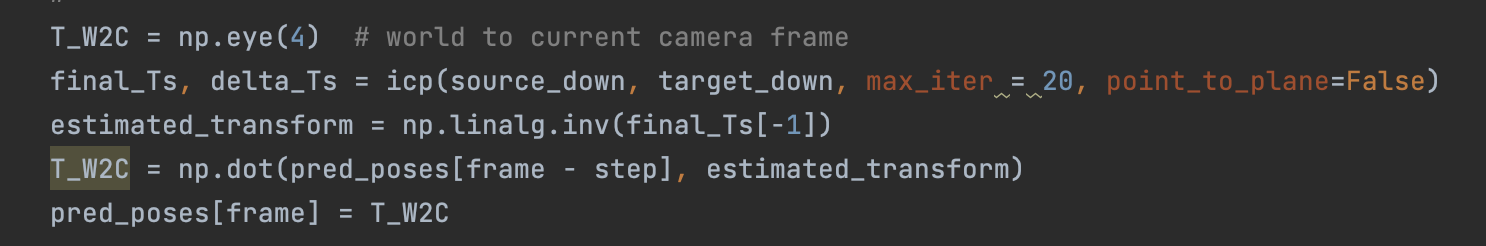
\includegraphics[width=0.3\linewidth]{fig/Q6code.png}
\end{center}
\begin{center}
    \small
    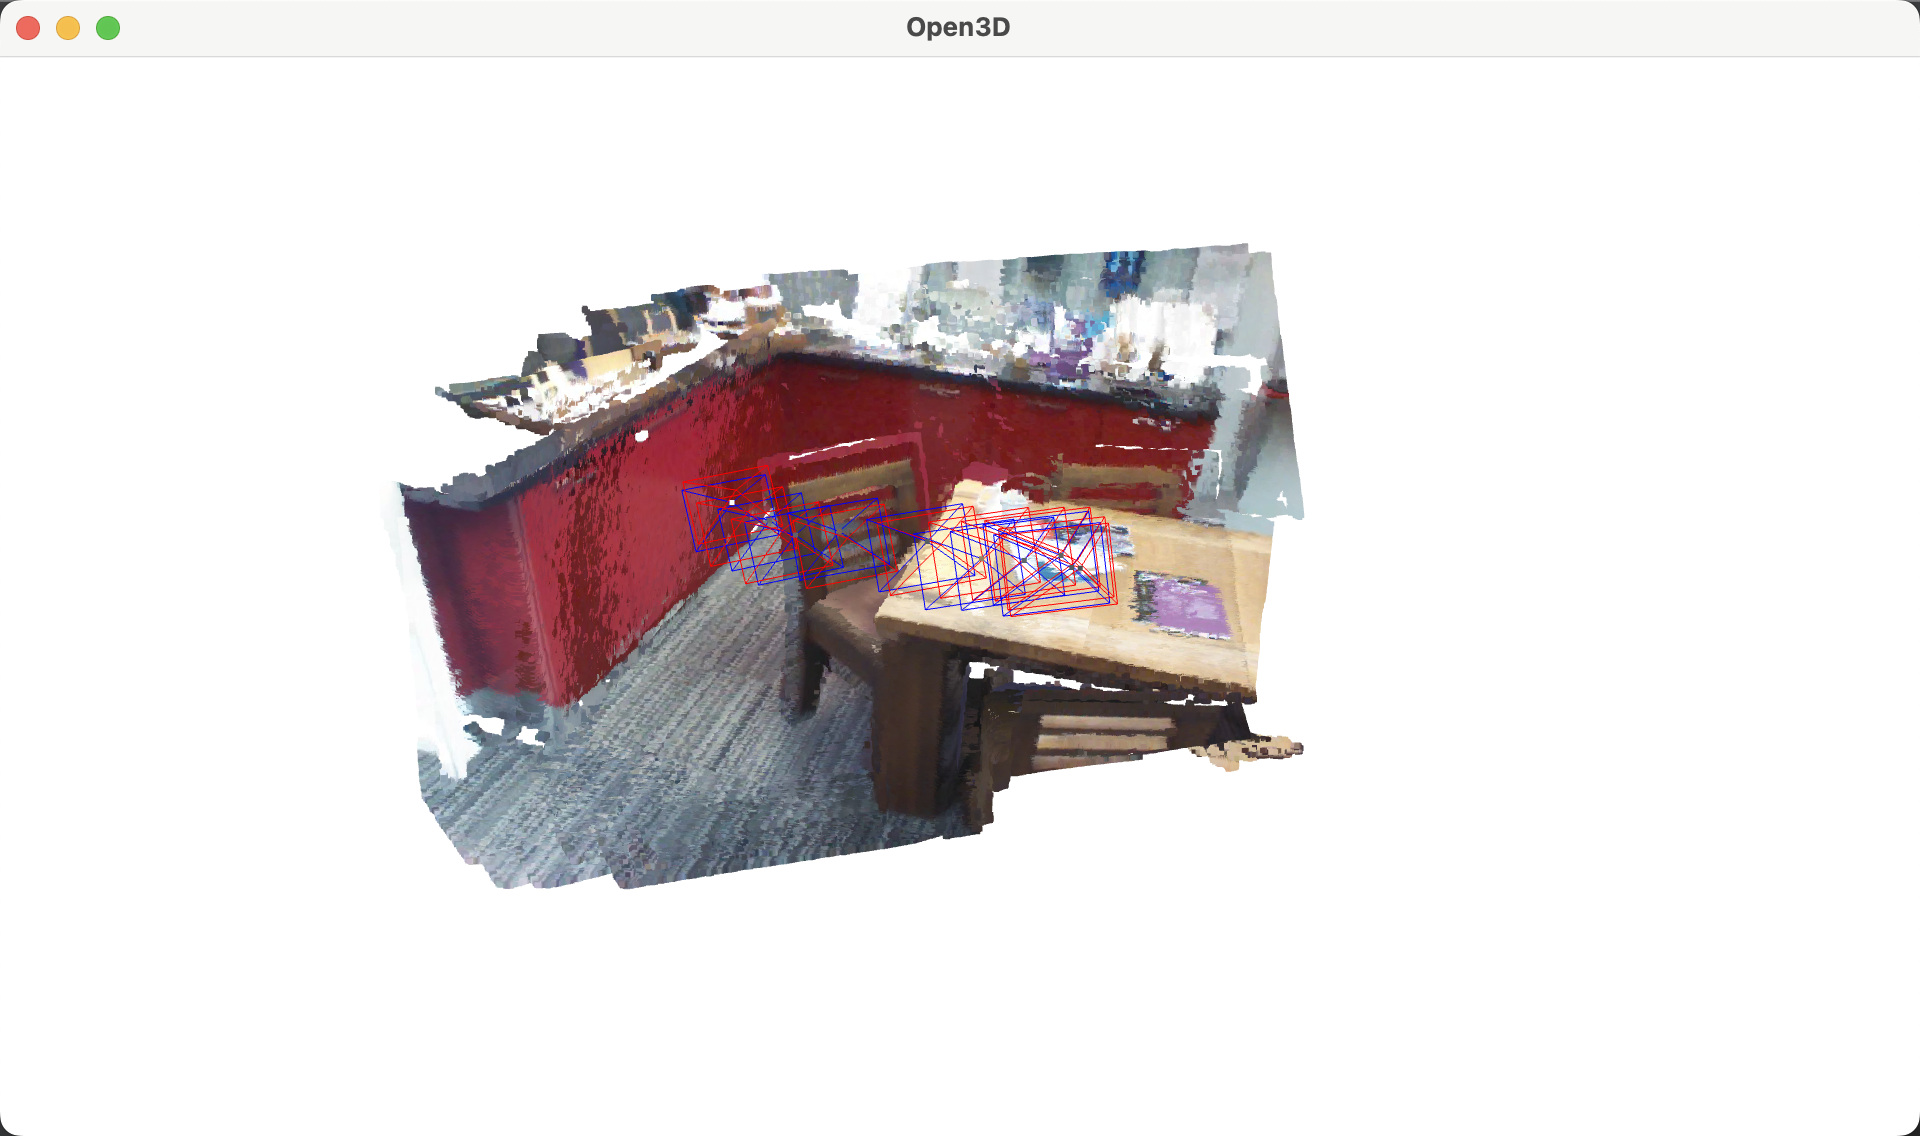
\includegraphics[width=0.3\linewidth]{fig/Q6output1.png}
    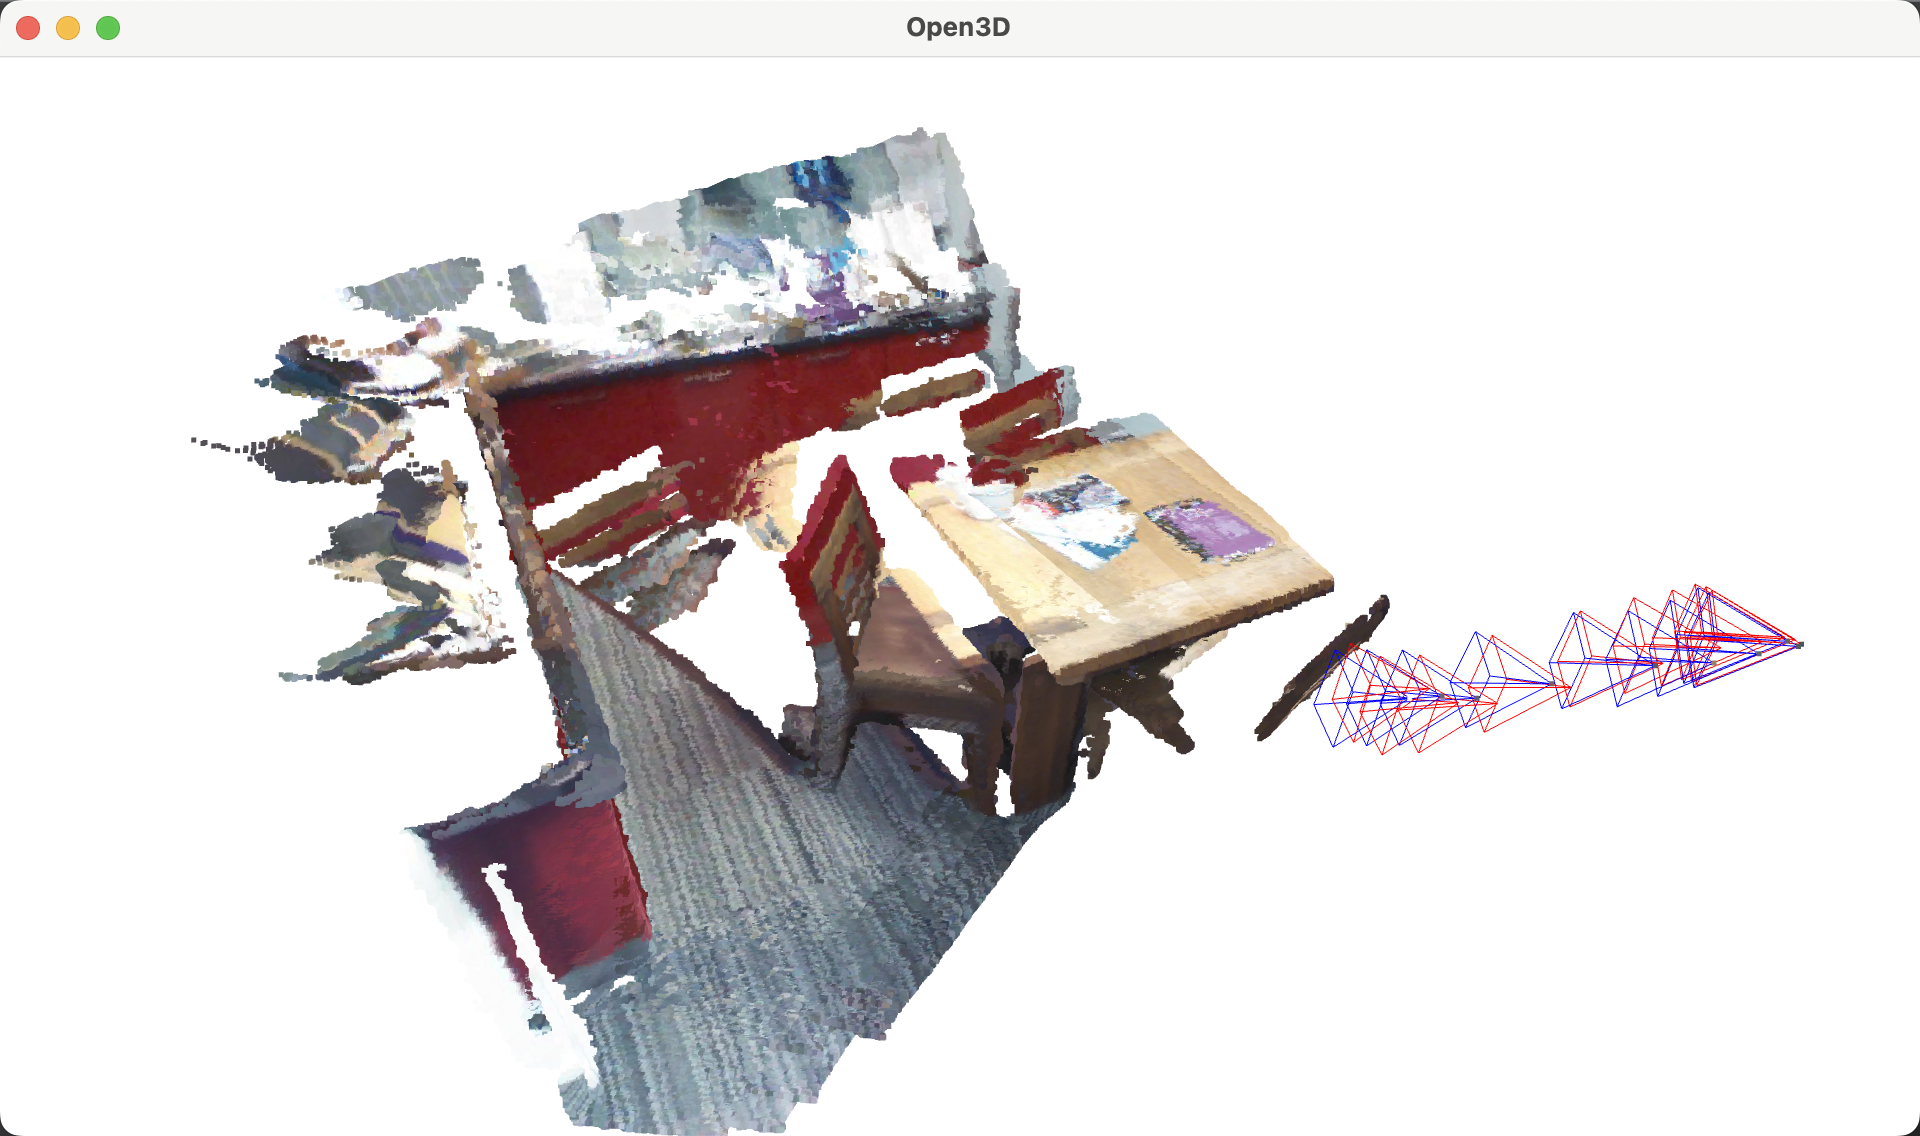
\includegraphics[width=0.3\linewidth]{fig/Q6output2.png}
    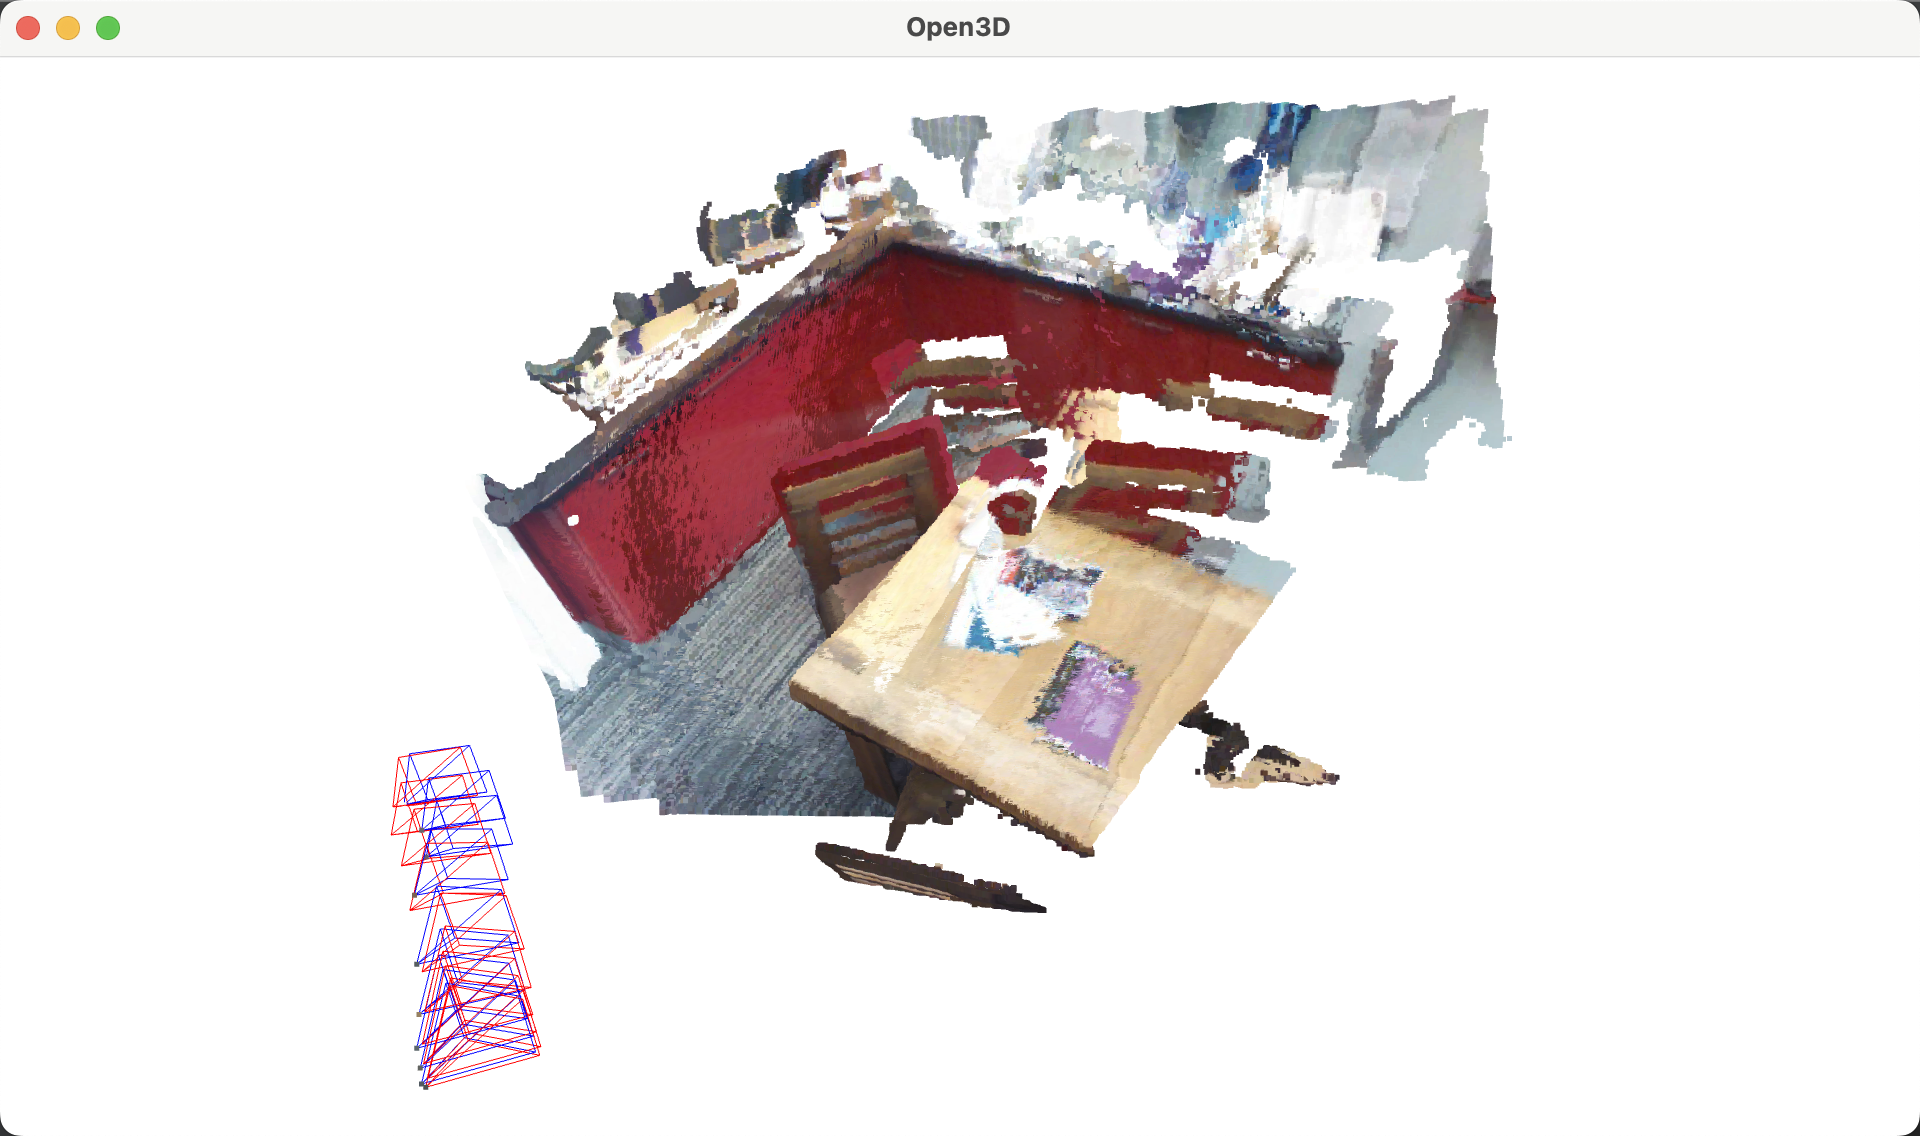
\includegraphics[width=0.3\linewidth]{fig/Q6output3.png}
\end{center}

\paragraph{Question 7 (Relative Trajectory Error) [2 pts]:}
Odometry cares about the accuracy of the relative poses. Due to the global pose drift, estimating the absolute pose error as we did for ICP might not be suitable for evaluating odometry. Thus, people use average relative pose error to measure the pose estimation accuracy for odometry/slam algorithms. Based on your implemented rotation and translation error estimation algorithm, please implement the following average relative pose error: (\href{http://www.cvlibs.net/publications/Geiger2012CVPR.pdf}{link} eq. 2 and eq. 3). Please visualize the estimated trajectory and ground-truth trajectory and report the error. 

\textbf{Answer: }The Rotation/Translation Error: 
$$\begin{bmatrix} 0.01101365 & 0.01668117 \end{bmatrix}$$
The estimated trajectory and grounnd-truth trajectory are shown in Q6.

\paragraph{Question 8 (Pose Graph Optimization) [2 pts]:}
So far, we have been only leveraging the relative transformation between adjacent frames. Absolute poses in global space are computed by accumulating the relative transformations. Do you think this is the best idea? What if there is one pair with a catastrophic alignment error? Given the odometry pose estimation of frame 0 and frame 40,
do you anticipate that they will be consistent with directly running ICP estimation between their corresponding point cloud? In this question, you will leverage a tool called pose graph optimization to help with the challenge. The general idea is simple: each frame's pose is a node in this graph, and any frames could be connected through an edge. On each edge, we define a cost measuring the agreement between the relative pose estimate between the two nodes and their pose estimation. By minimizing the energy, we are promoting global consistency across all the frames. More guidance is provided in the code.

\textbf{Answer: }The reult of pose graph optimization are shown as follows:
If I use all optimized estimate camera to unproject the 3d point cloud, the result is shown as follows:
\begin{center}
    \small
    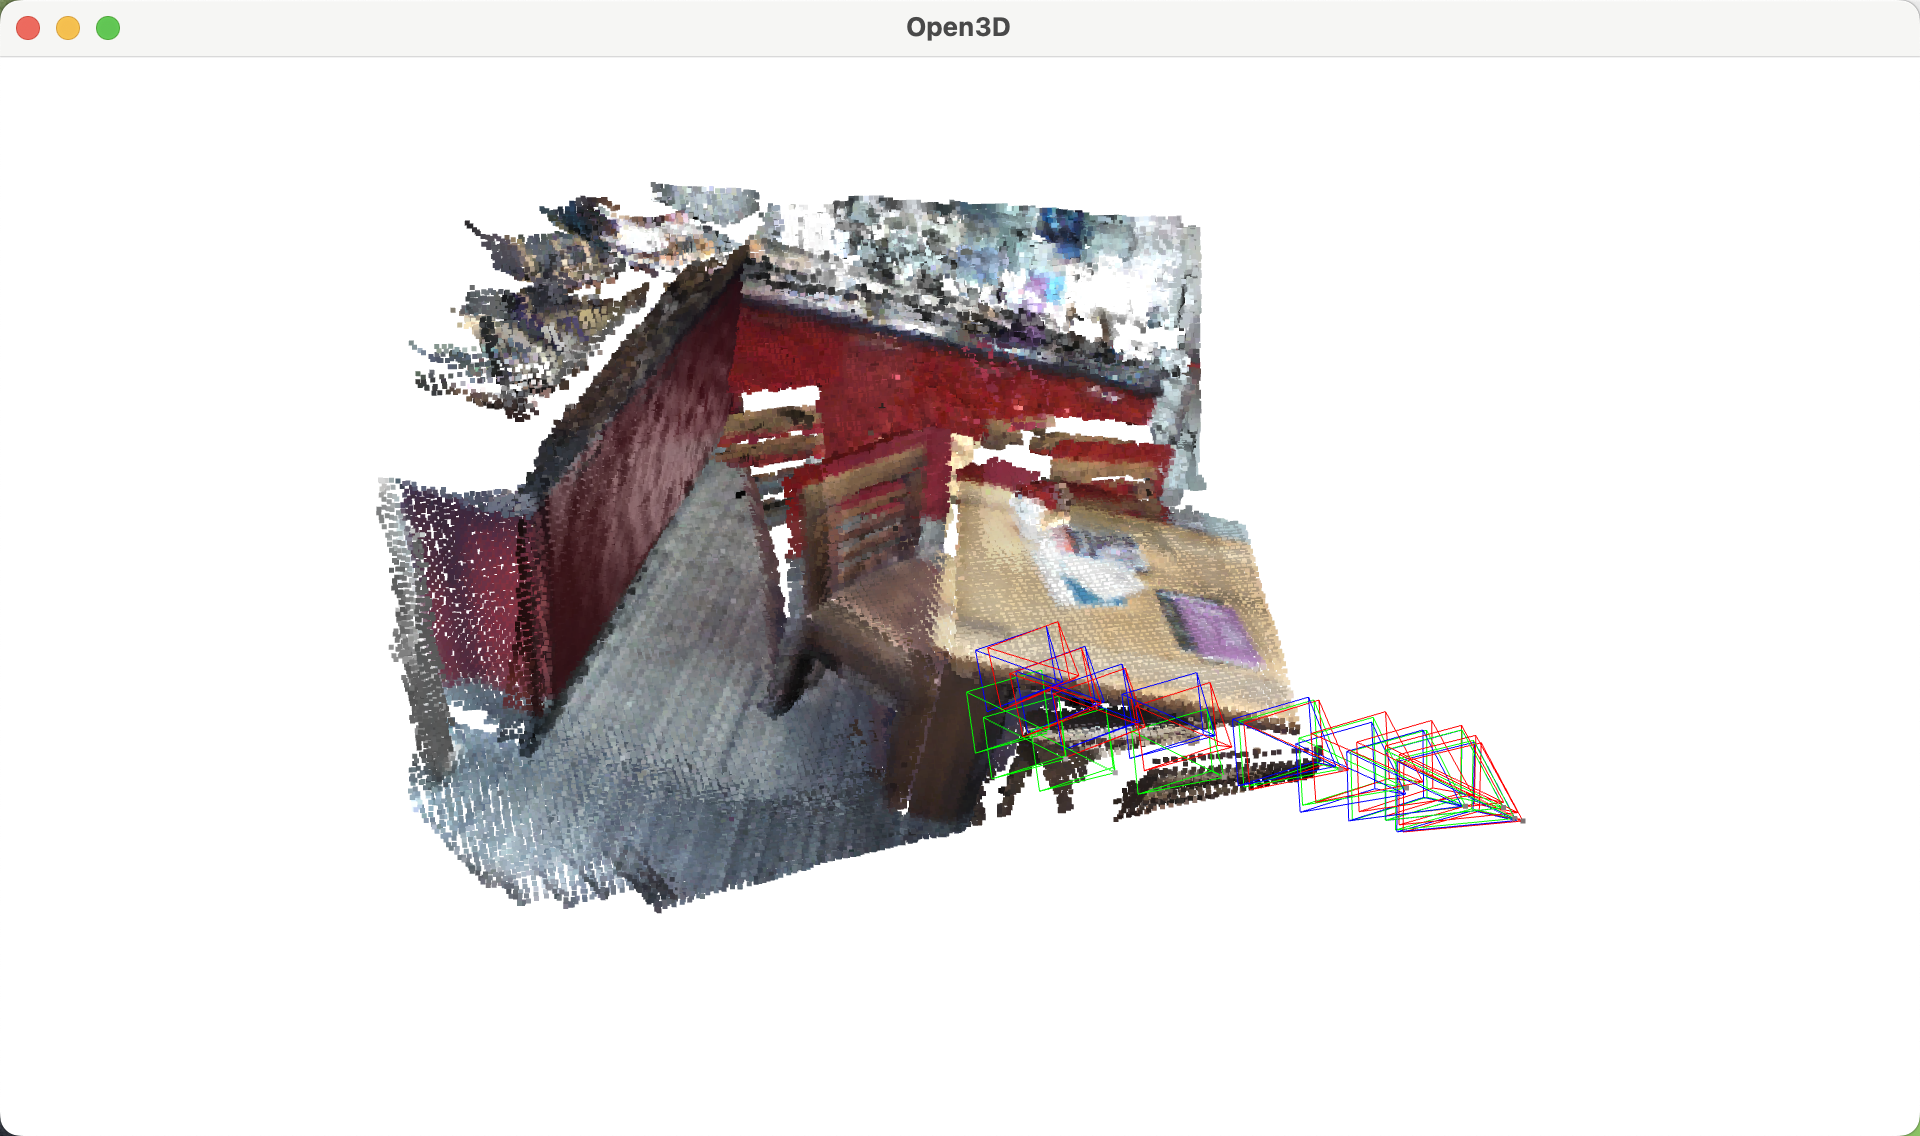
\includegraphics[width=0.3\linewidth]{fig/Q8-1output1.png}
    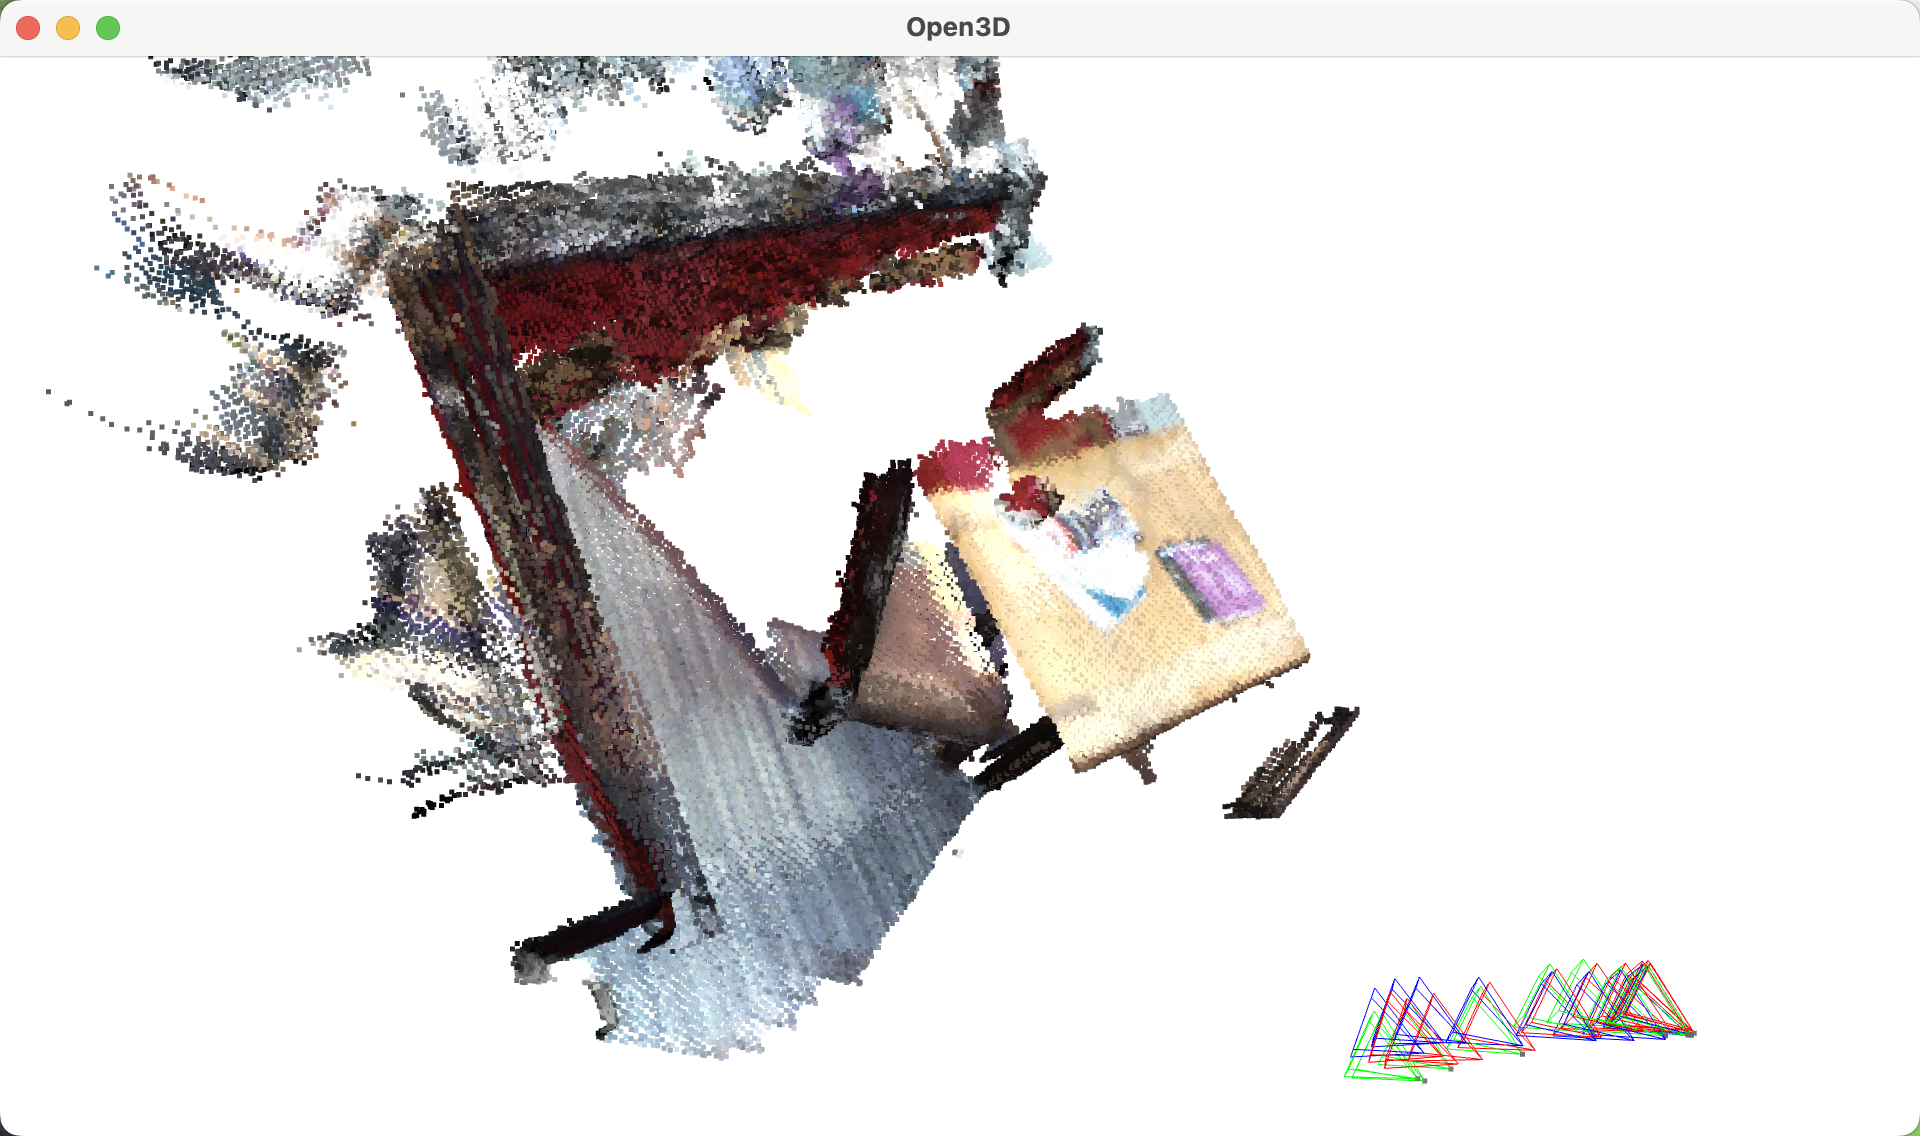
\includegraphics[width=0.3\linewidth]{fig/Q8-1output2.png}
\end{center}
After elimate those perspective with bad unproject result, the 3d point cloud restruction result is shown as follows:
\begin{center}
    \small
    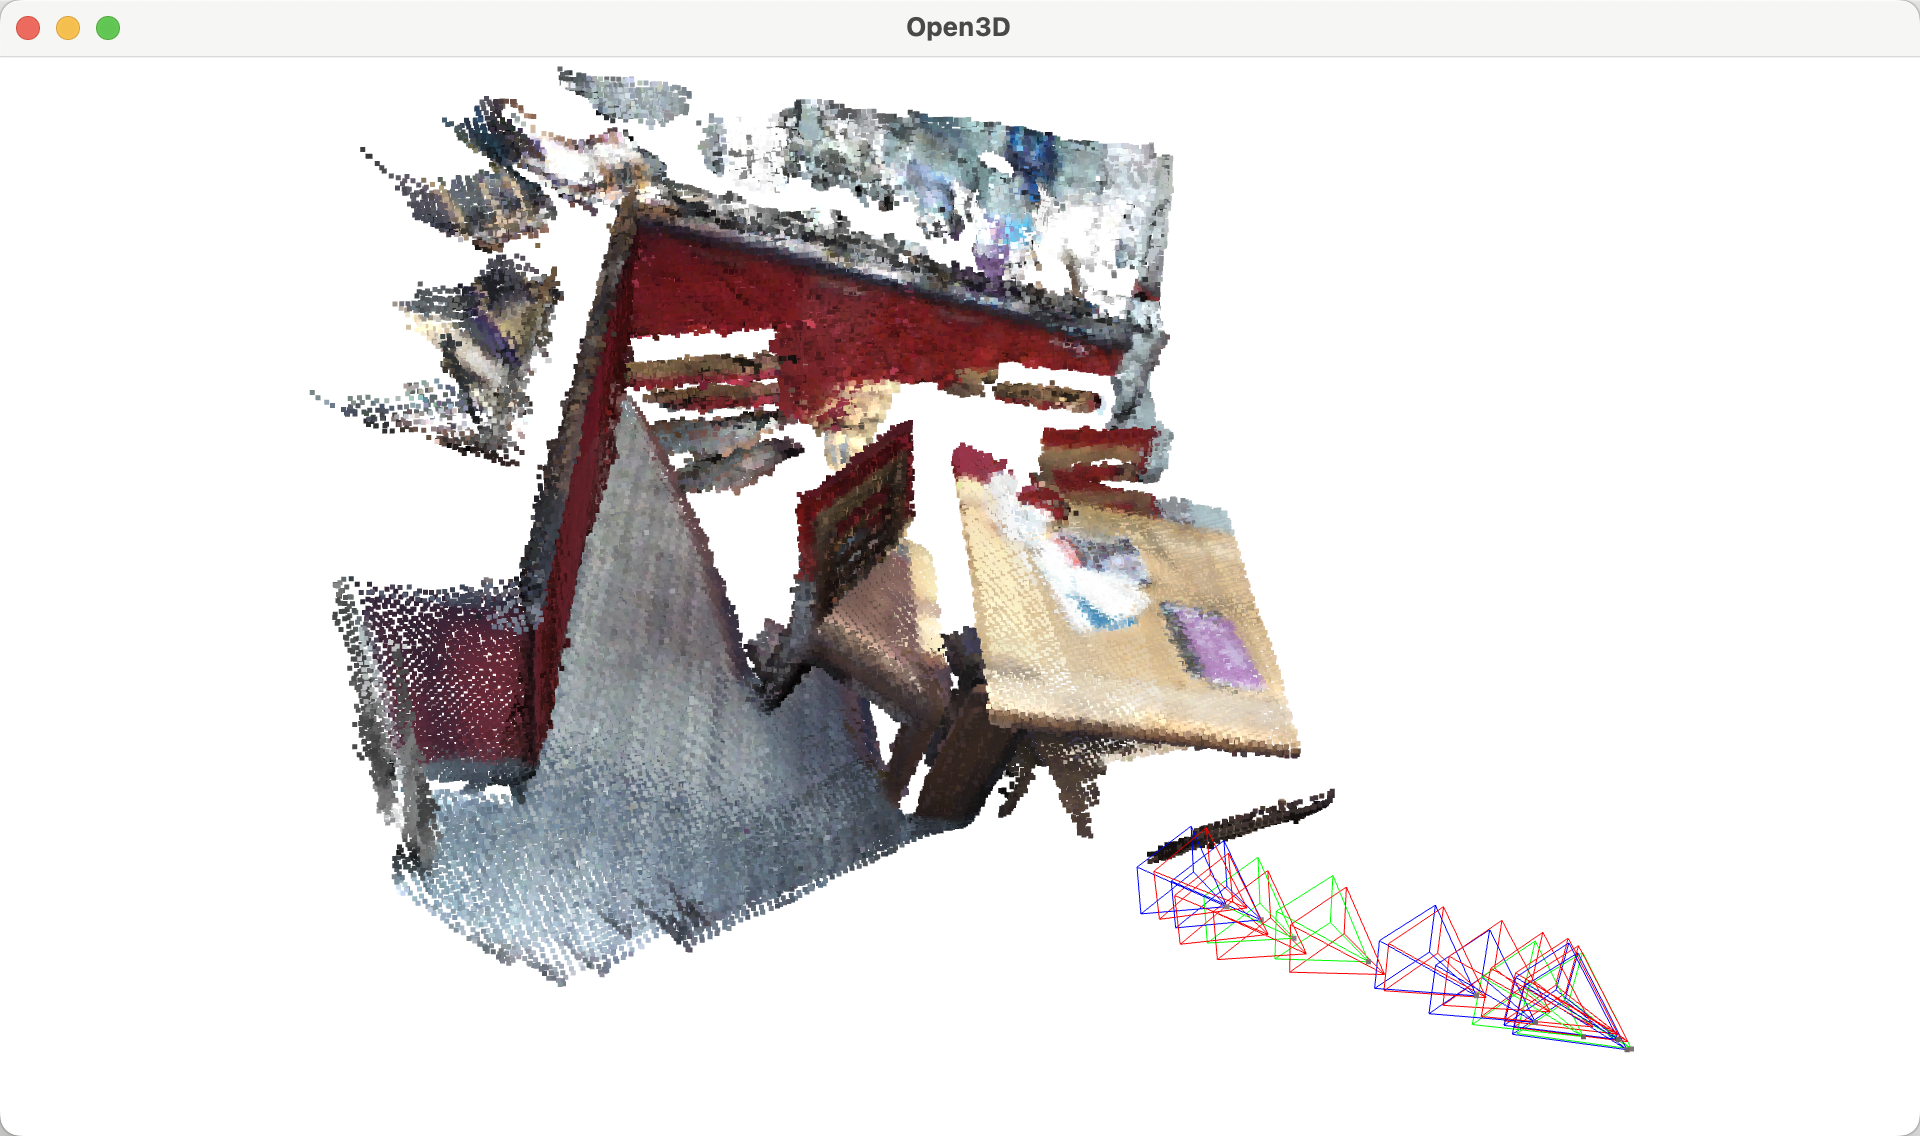
\includegraphics[width=0.3\linewidth]{fig/Q8-3output1.png}
    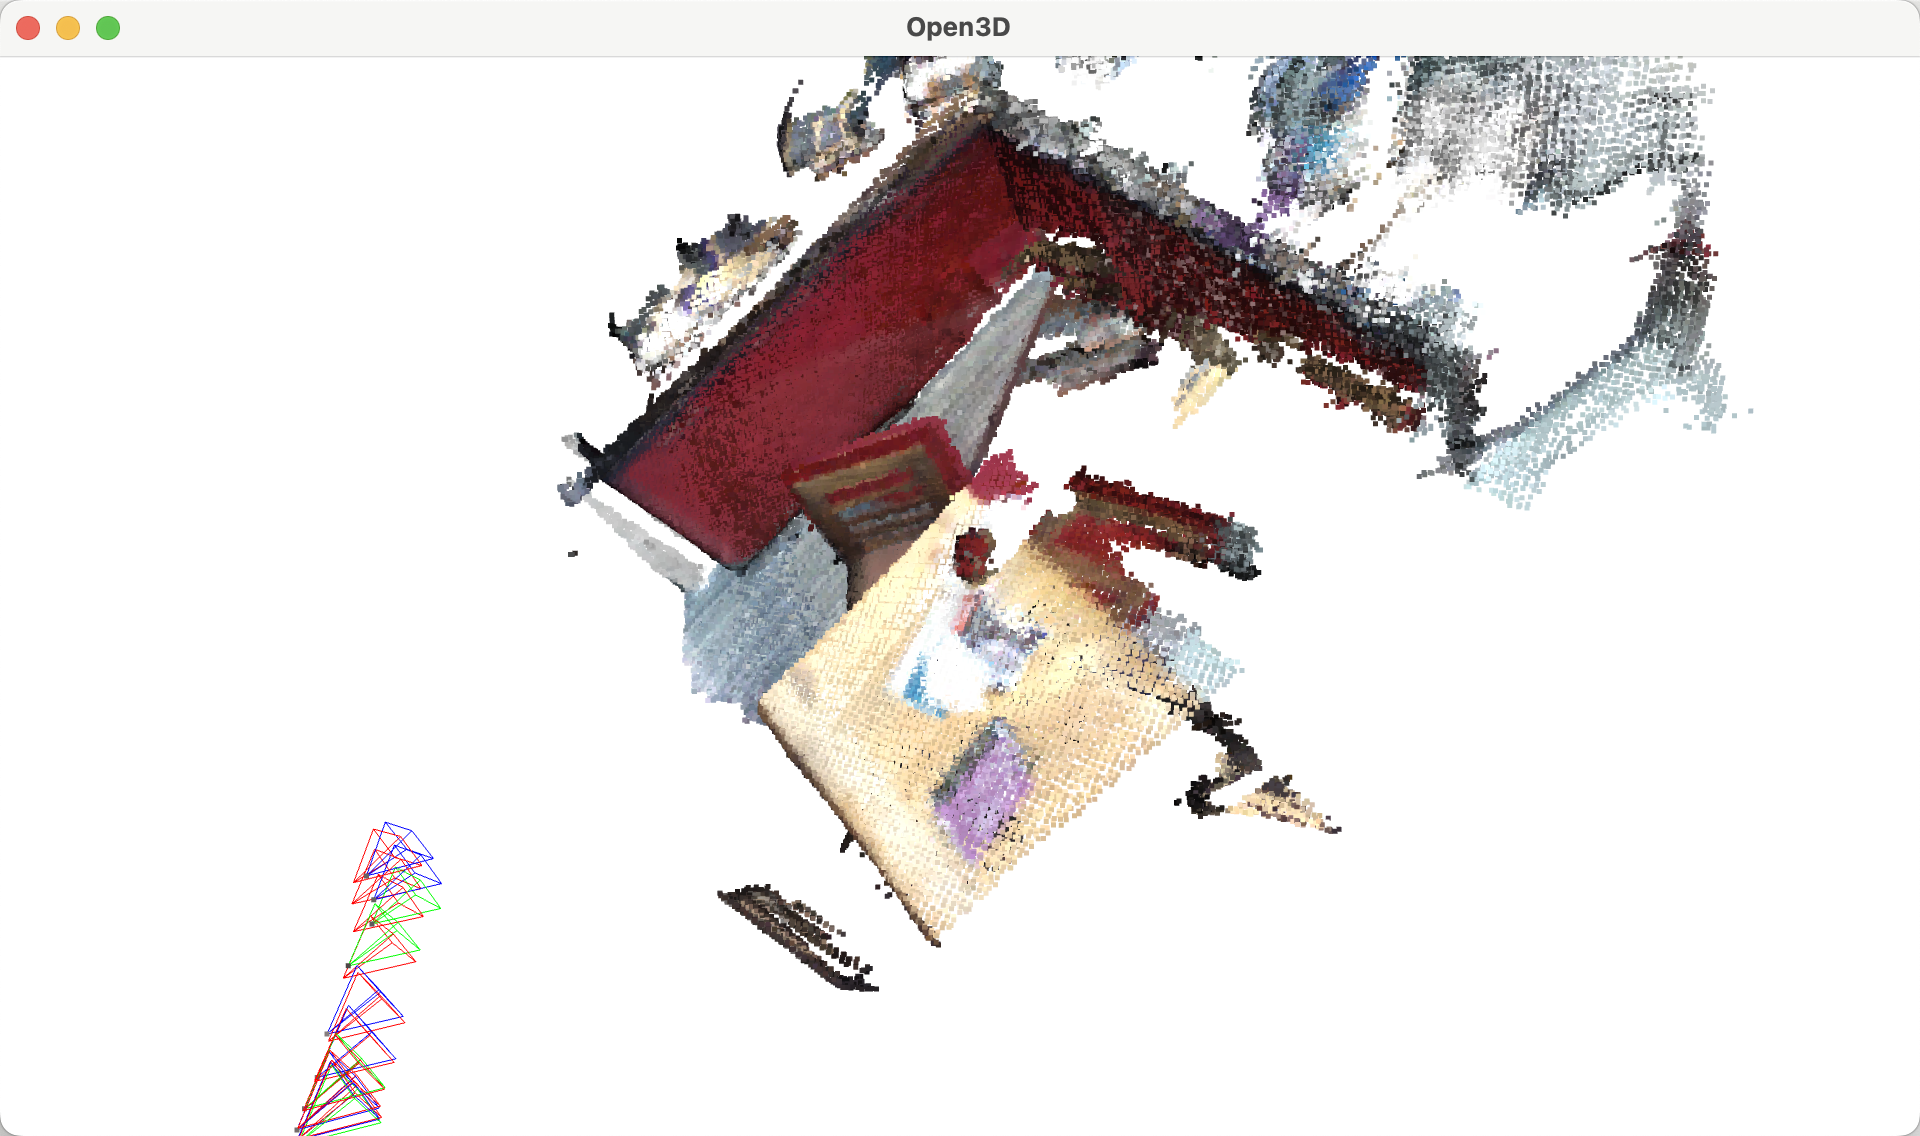
\includegraphics[width=0.3\linewidth]{fig/Q8-3output2.png}
    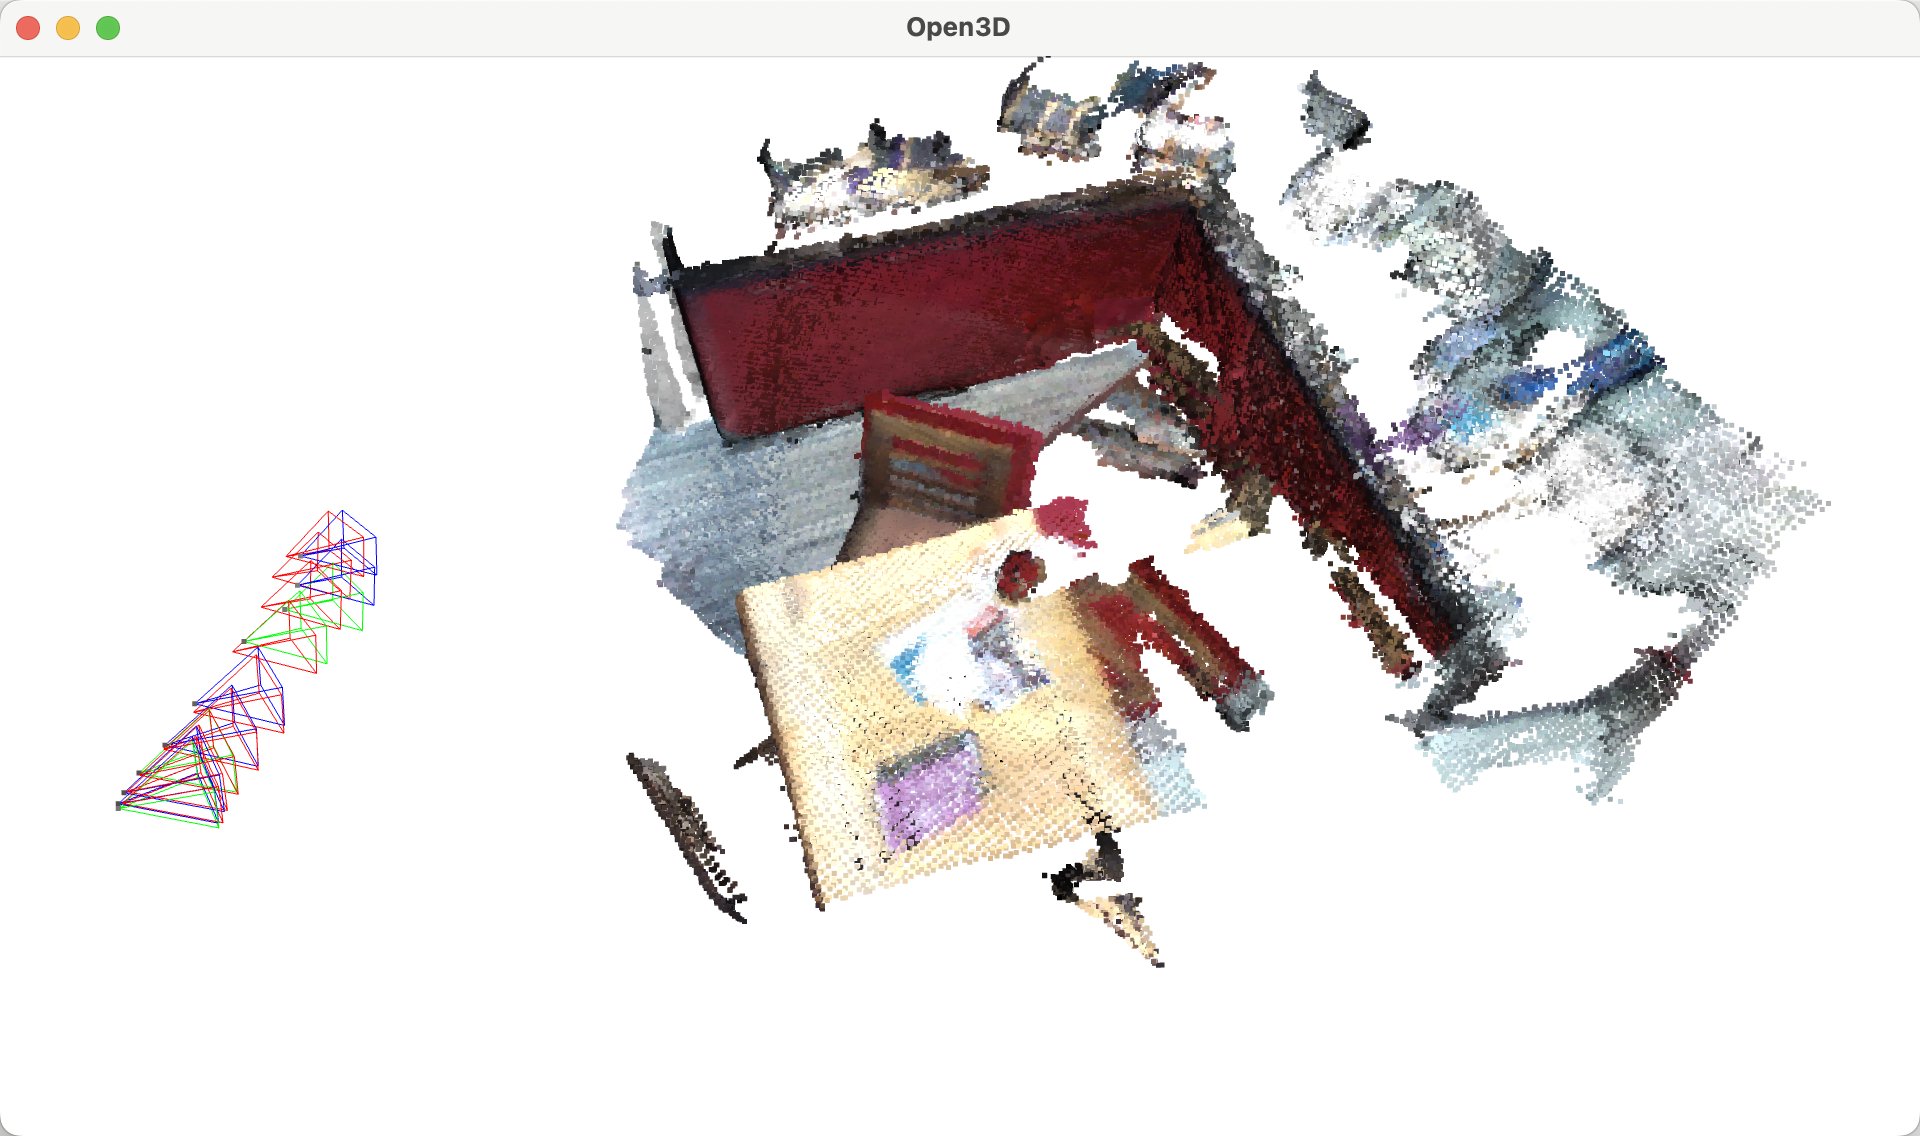
\includegraphics[width=0.3\linewidth]{fig/Q8-3output3.png}
\end{center}

\section*{Mapping (Bonus 3pt)}

We believe you have a great camera trajectory estimation now. This bonus question will leverage the well-aligned camera trajectory and build a 3D map of the room. The general idea is to leverage volumetric fusion, described in KinectFusion paper and covered in our lecture. The key is to incrementally update the signed distance values for each voxel in the volume if a new depth frame comes. Try to fuse the color and depth into the volume and use a marching cube to get the extracted mesh. Leveraging existing volumetric fusion functions will not count. That being said, you could use them as a sanity check. You are allowed to use the GT camera poses. Try your best to get visually appealing results. We will choose the top solution and announce them in the class. 
\end{document}. 

\grid
\grid